\documentclass[12pt,a4paper]{report}
\usepackage{amsmath,amsthm,amssymb,graphicx,hyperref}
\usepackage[left=1.2in,right=1in,top=1in,bottom=1in]{geometry}
\usepackage[romanian]{babel}
\usepackage{algorithm}
\usepackage{algpseudocode}
\usepackage{listings}
\usepackage[utf8]{inputenc}
\usepackage[T1]{fontenc}
\usepackage{subcaption}
\usepackage{booktabs}
\usepackage{graphicx}
\usepackage{tabularx}
\usepackage[
    backend=biber,
    style=authoryear,
    maxcitenames=2,
    maxbibnames=99
]{biblatex}

\usepackage{pdfpages}
\usepackage{dirtree}

\addbibresource{mybib.bib}
%\usepackage{...insert other packages here...}
\newtheorem{thm}{Teorema}[section]
\newtheorem{lem}[thm]{Lema}
\newtheorem{cor}[thm]{Corolarul}
\newtheorem{prop}[thm]{Propozi\c tia}
\theoremstyle{definition}
\newtheorem{defn}{Defini\c tia}[section]
\theoremstyle{remark}
\newtheorem{rem}{Remarca}[section]
\newtheorem{exmp}{Exemplul}[section]

\def\contentsname{Cuprins}
\def\listfigurename{Lista figurilor}
\def\listtablename{Lista tabelelor}
\def\figurename{Figura}
\def\tablename{Tabelul}
\def\partname{Partea}
\def\chaptername{Capitolul}
\def\refname{Referin'te}
\def\bibname{Bibliografie} 
\def\appendixname{Anexa}

\begin{document}
\thispagestyle{empty}
\begin{center}
\begin{figure}[h!]
\vspace{-20pt}
\begin{center}

\includegraphics[width=100pt]{FI.png}
\end{center}
\end{figure}


{\large{\bf UNIVERSITATEA DE VEST DIN TIMIȘOARA

FACULTATEA DE INFORMATICĂ

PROGRAMUL DE STUDII DE LICENȚĂ: Informatică }}

\vspace{120pt}
{\huge {\bf LUCRARE DE LICEN\c T\u A}}
\vspace{40pt}


\vspace{150pt}
\end{center}


\vfill
\begin{center}
{\bf TIMI\c SOARA

2026}
\end{center}
\newpage
\thispagestyle{empty}
\begin{center}
{\large{\bf UNIVERSITATEA DE VEST DIN TIMI\c SOARA

FACULTATEA DE INFORMATIC\u A


PROGRAMUL DE STUDII DE LICEN\c T\u A: Informatică}}

\vspace{120pt}

\vspace{40pt}

{\huge {\bf Evaluarea mișcărilor în VR și depistarea dizabilităților}}
\vspace{150pt}
\end{center}

{\large\noindent{\bf COORDONATOR:\hfill ABSOLVENT:}

\noindent Prof. Dr. Frîncu Marc \hfill Soos Kriszta}

\vfill
\begin{center}
{\bf TIMI\c SOARA

2026}
\end{center}
\newpage
\normalsize{}
\section*{Abstract}

Virtual Reality is increasingly utilized in fields such as education and medicine. Studies have evidenced that it has the ability to induce neurological effects comparable to those generated by real-world experiences. As a result, it can serve as an important support tool for individuals with various types of disabilities, e.g., motor impairments, by providing an effective and non-intrusive rehabilitation approach. Through artificial intelligence, behavioral patterns in virtual environments can be determined and analyzed, providing further insight into patients’ well-being.
Therefore, the aim of this study is to investigate behavioral patterns based on virtual reality data from 19 subjects and correlate them with the subjects’ medical motor disability. Three distinct scenarios covering various locomotion systems (i.e., controller-based, eye movement-based, and static–no movement) are investigated with real-time data collected from the virtual environment. Dimensionality reduction via Principal Component Analysis is employed, followed by unsupervised learning using the K-means algorithm.
Results show that the proposed methodology successfully detected all participants presenting motor disabilities, accurately capturing their specific navigational limitations through quantifiable kinematic signatures. The behavioral variation scoring system produced a structured three-tier classification, with the two clinically confirmed atypical participants receiving scores of 1.000 and 0.875, clearly separated from the remainder of the cohort. However, highly energetic or spatially exploratory participants were occasionally misclassified as atypical, indicating that the current model cannot yet reliably distinguish between restriction-driven and engagement-driven behavioral variation. These findings demonstrate the potential of VR-based unsupervised behavioral analysis as a non-intrusive screening tool for motor impairments, while highlighting the need for a secondary interpretative layer to improve classification specificity.

\tableofcontents
\newpage

\chapter{Introducere}

% Motivare tematica, context
Realitatea virtuală are un rol esențial în domeniul IT, reușind să creeze o punte între acesta și diferite arii de interes precum activități care pun accent pe distracție conform \cite{Samadbeik2018}, educație potrivit \cite{Lege2020}, \cite{Powell2017} sau medicină după \cite{Szekely1999}. În această secțiune a lucrării accentul este pus pe ariile medicale care sunt influențate de VR, explicând modul în care realitatea virtuală poate ajuta recuperarea medicală, identificarea unor predispoziții medicale fără a provoca stres subiecților și efectele sociale pe care le poate avea interacțiunea cu acesta. 

În primul rând, înțelegerea efctelor realității virtuale asupra percepției umane este esențială. Prin lucrarea scrisă de \textcite{Angerbauer2024} este studiat impactul, atât al mediilor sociale, cât și al celor virtuale asupra psihicului uman. Studiul se bazează pe un joc care unește cele două medii, oferind oamenilor posibilitatea de a își afișa condițiile medicale prin intermediul unor avatari în diferite contexte sociale online. Rezultatele au fost atât experiențe bune, cât și experiențe neplăcute pentru oamenii cu dizabilități. Acest studiu are o relevanță semnificativă, deoarece ilustrează dificultățile sociale prin care trec persoanele cu dizabilități, cât și importanța influenței realității virtuale care poate avea efecte aproape identice cu lumea reală. Astfel, puterea de imersiune pe care o exercită mediile virtuale este o unealtă remarcabilă care poate fi aplicată în multiple arii. 

Articolul scris de \textcite{Kober2022} urmărește evidențierea diferențelor de unde neurologice stocate printr-un sistem BCI (Brain-Computer Interface) în funcție de scenariul la care este supus individul. Astfel, în articol se înregistrează date de la diferiți subiecți în trei scenarii, realizând aceleași mișcări cu: mâinile reale, mâini abstracte reprezentate prin realitatea virtuală, și varianta cu aspect real a mâinilor asbstracte. Studiul arată că realitatea virtuală reușește să provoace unde neurologice într-un mod foarte asemănător procesului prin care aceste unde se nasc prin interacțiunea cu realitatea, dacă scenariul este apropriat vizual de realitate. Articolul realizat de \textcite{Fregna2025} aduce și mai multă claritate asupra acestui aspect.  Conform autorilor, există mai multe tipuri de nivel de imersiune pe care le poate experimenta utilizatorul: non-imersiv, semi-imersiv și imersiv. Cu cât gradul de imersiune este mai mare, cu atât rezultatele obținute pentru recuperarea pacienților sunt mai bune. În studiu se discută obstacole depistate în recuperarea prin realitatea virtuală. La pacienții care sunt afectați puternic de oboseala cauzată de scleroza multiplă, apar incompatibilități cu mediul virtual, deoarece oboseala afectează gradul de imersiune resimțit de utilizatori. Cu toate acestea, subiecții testați au raportat experiențe pozitive în mediul virtual, acesta arătându-se util, chiar dacă în acest caz nu își atinge potențialul maxim.

Astfel, realitatea virtuală poate fi folosită pentru a stimula unde neurologice cu scopul recuperării medicale. Următoarele studii reflectă rezultatele obțiunte în recuperări prin VR, pentru a înțelege importanța și aplicabilitatea acestui instrument din punct de vedere medical. Acest pas este esențial pentru trecerea în tematica specifică abordată de câtre prezentul document. 

Studiul realizat de \textcite{Saeed2025} ilustrează performanța atinsă prin utilizarea realității virtuale în procesul îmbunătățirii mișcării și al reducerii durerilor la copiii cu dizabilități la membrele inferioare, atrăgând atenția la faptul că realitatea virtuală poate fi mai bună decât abordarea tradițională în acest tip de context, din punct de vedere funcțional și psihologic. Un articol care pune accentul și mai mult pe caracterul neintruziv al mediilor VR este elaborat de \textcite{Tokarskaya2026}, care are în prim-plan testările cognitive la copii. Pentru copiii cu TSA (tulburări de spectru autist) testările tradiționale pot fi stresante, deoarece simptomul duce la bariere sociale, anxietate în medii noi și senzivitate senzorială. Prin metoda realității virtuale au fost colectate rezultate similare cu testările pe hârtie sau PC. Aspectul important de menționat din acest studiu este acela că participanții au raportat semne de siguranță și dorința de a repeta experiența, studiul concluzionând în faptul că VR-ul crează un mediu prietenos și detensionat pentru copiii cu TSA, eliminând discomfortul testărilor tradiționale. Aceste exemple atrag atenția la ideea că mediile virtuale deschid o cale sigură și prietenoasă pentru diagnosticarea pacienților cu diferite tulburări. 

De asemenea, obiectivitatea în depistarea afecțiunilor este un aspect care poate fi îmbunătâțit de technologie. Articolul scris de \textcite{Kim2023} prezintă problematica identificării persoanelor cu Deficință Cognitivă Ușoara (MCI), indicator al afecțiunii Alzheimer. Acest studiu se bazează pe testarea pacienților apelând la un mediu virtual cu scopul de a plasa comenzi la un chioșc. Rezultatele au arătat un comportament diferit din partea celor cu MCI. Aceștia au fost mai lenți, prezentând dificultăți de concentrare prin privire, necesitînd mai mult timp pentru a completa sarcina și având un număr mai mare de greșeli. Un experiment similar este descris în articolul scris de \textcite{Park2025}. Asemănător cu studiul anterior, în acesta cerința era de a sorta haine.  Studiul subliniază faptul că rezultatele VRST (Virtual Reality Stroop Test) au prezentat o corelare cu testele clinice standard, marcării derivați din VR depâșind testul tradițional MoCA (\textcite{Julayanont2013}). Abordarea implementată susține faptul că persoanele ce prezintă MCI au deficite de memorie și inhibiție.

Studiile nu se opresc la identificarea anumitor dizabilități prin VR. Articolul scris de \textcite{Moskiewicz2025}  prezintă aplicabilitatea realității virtuale în cazul pacienților care au suferit accidente vasculare cerebrale (AVC) urmate de paralizie. Realitatea virtuală este esențială datorită faptului că oferă date în timp real despre reacțiile și comportamentele pacientului. Prin acest mod, procesul învățării motorii este eficentizat, fiind o abordare sigură și neintruzivă. Conform articolului menționat, realitatea virtuală reprezintă un instrument care poate fi utilizat ca o îmbunătățire pentru fizioterapie, această combinație a practicii tradiționale și al realității virtuale având rezultate semnificative.

Astfel, este demonstrat faptul că realitatea virtuală este esențială datorită efectelor psihologice pe care le poate crea, similare cu efectele produse de realitatea însăși. Pentru pacienți reprezintă un mediu noninvaziv prin care aceștia pot fi diagnosticați, un ajutor considerabil în procesul de recuperare, dar și un spațiu unde pot întâlni persoane aflate în același context social. Pentru medici și oameni de știință realitatea virtuală este un instrument care poate duce la diagnostice obiective, neinfluențate de aspecte ce țin de performanța umană, extinzându-le capacitățile omenești.

Cu toate acestea, identificarea dizabilităților motorii prin realitatea virtuală este un subiect mai puțin experimentat și documentat, față de alte arii de cercetare în plină evoluție. Existența unui astfel de studiu este esențială, deoarece deschide calea spre noi practici și mecanisme de monitorizare și adaptare la nevoile persoanelor cu dizabilități, precum jocurile serioase.

% Probleme teoretice/ aplicative discutate in lucrare


\section{Obiectivele urmărite}
% Obiective urmarite/ atinse
În acest context, lucrarea ”Evaluarea mișcărilor în VR și depistarea dizabilitățlor” își propune să studieze interacțiunea oamenilor cu dizabilități cu mediul virtual. Scopul principal este de a observa diferențe în comportament în mediul virtual între participanții cu dizabilități motorii și cei tipici. Obiectivul final fiind cel de distincție între persoane cu dizabilități motorii și cei sănătoși, doar prin prisma comportamentelor înregistrate în mediul virtual.


% Descrierea informala a solutiei
\section{Descrierea soluției}

Pentru a atinge obiectivul propus, proiectul are la bază un joc VR. Acesta presupune explorarea clădirii sediului Universității de Vest din Timișoara. Participanții sunt testați în trei scenarii cu grade de libertate locomotorie diferite pentru a simula imposibilitatea de mișcare. Prin această abordare se analizează nu doar comportamentele utilizatorilor în realitatea virtuală, dar și modul lor de gestionare a situațiilor dificile. Datele stocate sunt procesate și se stabilesc caracteristicile comportamentale pentru fiecare utilizator. Prin diferiți algoritmi de reducere dimensională și grupare a punctelor în spațiu, se face distincția între comportamente. Pentru un nivel de complexitate avansat se calculează diferite distanțe între punctele din spațiu și se crează un scor de consistență pentru fiecare utilizator. Ca ultim pas de analiză, se calculează un scor final și se împart utilizatorii pe diferite grade de atipicitate în funcție de scorul primit. O parte esențială a abordării propuse este generarea de imagini vizuale. Acestea sunt de mai multe tipuri ilustrând mișcarea fiecărui utilizator pe scenarii individuale sau grupate. Ele au scopul de a evalua analiza numerică anterioară și de a contribui la concluzia finală legată de tipul și motivul din spatele unui comportament anume.


% Pentru a atinge obiectivul propus, proiectul are la bază un joc VR. Acest joc îi supune pe participanți la explorarea anumitor holuri din clădirea Facultății de Informatică, din cadrul Universității de Vest din Timișoara. Trei scenarii sunt parcurse în mod aleatoriu de câtre subiecți. Scenariul notat prin litera "A" îi îngrădește pe utilizatori, permițându-le să exploreze spațiul doar cu privirea. Motivația este de a simula incapabilitatea de mișcare, căutând comportamente de agitație, plictiseală sau exasperare la participanții fără dizabilități motorii, ei nefiind obișnuiți cu astfel de limitări. Scenariul notat prin litera "B", propune descoperirea hărții prin utilizarea privirii. Utilizatorul se poate deplasa doar prin țintirea cu privirea a două tipuri de blocuri abstracte, care permit mișcarea în direcția lor sau rotirea la 45 de grade. Acest scenariu renunță la limitarea impusă de scenariul anterior, însă îngreunează semnificativ traversarea holurilor, aspect mai puțin întâlnit de persoanele fără dizabilități motorii. Ultimul scenariu, notat cu "C" utilizează controllerele specifice echipamentelor VR, așteptând un comportament normal, calm, fără reacții negative din partea utilizatorilor tipici. 
% În urma colectării datelor de la utilizatori, acestea sunt procesate și se crează imagini vizuale reprezentând comportamentele acestora. De asemenea, se cere feedback prin formular în urma fiecărui scenariu, prin care utilizatorii împărtășesc informații despre modul în care s-au simțit încercând să exploreze scenariul. 

Astfel, totalitatea reprezentărilor vizuale, statisticilor și feedbackului utilizatorilor reprezintă soluția pentru a observa diferențe comportamentale în VR între persoane cu dizabilității motorii și perosoane tipice.

% Relevanta rezultatelor
\section{Relevanța rezultatelor}
Rezultatele sunt considerate relevante, deoarece abordeaza o problematică de bază și pot fi utilizate drept punct de pornire pentru dezvoltări ulterioare. 
Rezultatele au arătat că implementarea unor tehnici de învățare automată nesupravegheată poate reprezenta o modalitate de identificare al anomaliilor comportamentale în spațiul VR. Mecanismul creat reușește să detecteze toate comportamentele atipice care sunt în corelație cu diagnostice clinice reprezentând dizabilități motorii și poate fi baza pentru cercetări avansate.

% Contributia autorului
% \section{Contribuția autorului}
% % Contribuția autorului se concentrează în partea analizei datelor. Începând de la generarea reprezentărilor vizuale, compararea acestora, până la analiza diferențelor comportamentela și reacțiilor atipice. %TODO: Scurta descriere comparativa cu ce exista deja pe aceasta tematica
% Prin comparație cu abordările actuale, proiectul prezent deschide o nouă cale spre analiza comportamentelor în VR. În articolul scris de \textcite{AlcanizRaya2020} se prezintă o aborsare pentru a diferenția comportamentele celor cu tlburare de spectru autist de comportamentele persoanelor tipice. Aspecte care nu se regăsesc în abordarea propusă de prezentul proiect sunt folosirea unui sistem de tip  CAVE (Cave Assisted Virtual Environment), camera virtuală având dimensiunea de 4x4x3 metrii, cu trei proiectoare, alături de sisteme audio și olfactive. De asemenea, mișcărilor au fost captate prin utilizarea unei camere Intel RealSense. Printre asemănări se numără calcularea distanței (distanța Euclidiană) și utilizarea algoritmului PCA (Principal Component Analysis). Cu toate acestea, în studiul realizat de \textcite{AlcanizRaya2020} accentul se pune pe modelul de clasificare SVM (Support Vector Machine). Pentru evaluarea acurateții au fost folosite testările tradiționale, iar rezultatele au fost comparate cu cele obținute prin aplicarea realității virtuale.

% Un alt articol relevant în aria de aplicabilitate al studiului prezent, este elaborat de\textcite{Afdideh2025}. Acest studiu are ca și element specific analiza undelor neurologice, care necesită echipamente specifice. Aceasta este diferența principală între proiectul discutat în acest articol și studiul realizat de \textcite{Afdideh2025}. În ceea ce privește tehnicile de procesare și învățare automată, studiul folosește o abordare focalizată pe specificitățile subiecților. Această abordare include utilizarea MAV (Mean Absolute Value), FFT (Fast Fourier Transform), AR (Coeficienți Autoregresivi) și Puterea Benzii. Clasificatorul utilizat este de tip Linear Discriminant Analysis. Validarea presupune tehnica Cross-Validation. 

% Un alt articol de precizat este cel scris de \textcite{Vlasiu2024}, având ca și scop identificarea persoanelor cu dizabilități mentale prin intermediul realității virtuale. Experimentele au fost realizate cu ajutorul echipamentului Oculus MetaQuest 2, participanții fiind expuși la diferite scene virtuale interactive, precum camere cu obiecte sau medii naturale simulate. Datele colectate au constat în poziția capului și direcția privirii, înregistrate periodic pe durata sesiunilor VR. Studiul se bazează pe algoritmi precum Support Vector Machine (SVM), Decision Trees (DT) și Random Forest (RF), implementați prin biblioteca Scikit-Learn din Python. 

% În comparație cu aceste studii, proiectul actual folosește echipament VR reprezentat prin cască și controllere de tip Oculus MetaQuest2. Algoritmii se bazează pe extragerea informațiilor colectate prin mișcarea capului. Din datele colectate se crează parametrii utili pentru analiza mișcărilor prin apel la inginera datelor. Abordarea presupune o modalitate de clasificare ierarhica precoce, care să ofere o viziune generală asupra comportamentelor depistate în VR, urmată de o analiză mult mai complexă. Cea de a doua abordare presupune utilizarea PCA și clusterizare de tip k-means, precum și calcularea a două tipuri de distanțe, care, împreună cu un scor de conistență rezultă scorul final de atipicitate pe baza căruia participanții sunt categorizați. Un aspect important este reprezentat de vizualizarea traseelor făcute de câtre utilizatori prin ploturi generate. Validarea se face prin compararea datelor rezultate prin clasificarea automată, cu datele colectate prin formular despre situația medicală a fiecărui participant.

% Astfel, abordarea prezentată în acest document descrie o nouă modalitate de analiză a comportamentelor în VR, față de cele câteva abordări existente în acest domeniu.

% Structura lucrarii 
\section{Structura lucrării}

% adaugă context despre aplicația VR, modul în care a fost structurat, toate datele care sunt stranse prin aplicație.
Partea aplicativă al studiului urmează o traiectorie clară și structurată. Datele de mișcare sunt înregistrate pe un interval de timp exact pentru fiecare participant și salvate în fișiere separate. Acestea sunt curățate și validate, urmând a fi creat profilul de caracteristici pentru fiecare utilizator. După acest pas se reduce spațiul de dimensionalitate și se grupează comportamentele în baza similarităților. Se calculează distanțe specifice între puncte și se creează un scor final pe baza căruia utilizatorii sunt împărțiți în diferite grade de atipicitate. 

Punctele cheie ale pipeline-ului sunt reprezentate de următoarele module:

\begin{itemize}
    \item \textbf{Configurarea și Setările Inițiale}: Acest modul are rolul de a gestiona setările globale ale proiectului, precum și de a defini parametrii de prag pentru clasificare. Definește numărul minim de scenarii necesare pentru analiză, rata maximă de fișiere corupte acceptată, ponderile pentru calculul scorului final și praguri pentru clasificarea atipicității. Aceste setări sunt esențiale pentru a asigura un proces de analiză consistent și adaptabil la diferite condiții ale datelor.
    \item \textbf{Nucleul de Procesare și Extracție}: Acesta este primul filtru prin care trec datele. Acesta se concentrează pe extragerea și curățarea coordonatelor spațiale. Transformă datele brute într-o serie complexă de indicatori comportamentali. Prin extragerea acestor caracteristici se va realiza gruparea în funcție de comportamente. Aceste funcții asigură un proces riguros de normalizare și validare matematică pentru a asigura stabilitatea analizelor ulterioare.
    \item \textbf{Motorul de Analiză și Clasificare}: Aceasta este etapa de analiză comportamentală și detecție a anomaliilor. Acest lucru se realizează prin implementarea tehnicilor de învățare nesupervizate. Pentru gruparea datelor se utilizează două abordări. Clasificarea ierarhică aglomerativăîmparte datele în 3 grupuri și generează diagrame ierarhice. Cea de a doua abordare presupune gruparea automată a punctelor apropiate și poate indica existența valorilor atipice. Se calculează un scor pentru a măsura gradul de asemănare dintre subiect și restul grupului, iar scorul final este calculat prin suma ponderată între distanța globală, anomalitatea statistică și diferența față de grup. Rezultatele numerice sunt transformate în etichete. 
    \item \textbf{Cadrul de Evaluare și Validare}: Pentru evaluarea modulelor create există teste unitare folosind date reale, pentru a asigura funcționarea corectă a algoritmilor. La nivel global, programul este validat prin compararea clasificărilor generate cu datele reale privind statutul persoanelor implicate în studiu, colectate prin acordul acestora, stocate în formă anonimă.
    \item \textbf{Instrumente de Vizualizare și Raportare}: Acest pas reprezintă implementarea funcțiilor pentru vizualizarea datelor, cât și generarea de rapoarte. Gruparea se realizează în două moduri: crearea clusterelor și calculearea statisticilor, și prin clusterizare ierarhică. De asemenea, în acest pas se realizează rapoartele comportamentale, care reprezintă o analiză suplimentară a comportamentelor.
    \item \textbf{Gestiunea Resurselor și Utilitare}: În acest pas se realizează organizarea datelor, consolidarea caracteristicilor și mentenanța sistemului. In acest pas, fișierele sunt organizate automat pe baza identificatorilor participanților, astfel încât toate datele asociate aceleiași persoane să fie grupate împreună. Apoi, informațiile provenite din mai multe scenarii sunt transformate într-un format unitar și compact, ușor de analizat ulterior. De asemenea, sistemul permite curațarea mediului de lucru prin eliminarea rapoartelor și imaginilor generate anterior, pentru a menține organizarea și a evita acumularea fișierelor inutile.
\end{itemize}

Schema de jos înfățișează structura exactă a codului implementat:\\
\newline

\dirtree{%
.1 PROIECT.
.2 config.
.3 disability\_config.py.
.2 core.
.3 analysis.
.4 clustering.py.
.4 disability\_engine.py.
.3 processing.
.4 data\_loader.py.
.4 feature\_extractor.py.
.2 data.
.3 ground\_truth.
.3 output.
.3 vr\_recordings.
.2 evaluation.
.3 ground\_truth\_handler.py.
.3 metrics.py.
.2 utils.
.3 file\_management.py.
.2 visualization.
.3 plotter\_3d.py.
.3 reports.py.
.3 scenario\_comparison.py.
.2 main.py.
}

% Caz de utilizare 

Următorul caz de utilizare prezintă fluxul după care a fost conceput sistemul descris:
\begin{itemize}
    \item \textbf{Preondiții:} Fișierele ce urmează a fi prelucrate să existe în folderul \\ data/vr\_recordings/. Acestea trebuie să respecte structura de forma unei liste de dicționare. Exemplu:  
    \begin{verbatim}
"Recordings": [
    {
        "ID": 0,
        "RealTimeTimestamp": "15/10/2025 - 10:59:50",
        "SceneTime": 0.7133399690055847,
        "HeadPosition": "(0.00, 1.20, -0.15)",
        "HeadRotation": "(0.00, 0.00, 0.00)",
        "HeadForward": "(0.00, 0.00, 1.00)",
        "LeftHandPosition": "(0.00, 1.20, -0.15)",
        "LeftHandRotation": "(0.00, 0.00, 0.00)",
        "LeftHandForward": "(0.00, 0.00, 1.00)",
        "RightHandPosition": "(0.00, 1.20, -0.15)",
        "RightHandRotation": "(0.00, 0.00, 0.00)",
        "RightHandForward": "(0.00, 0.00, 1.00)"
    }
]
\end{verbatim}
    Denumirea fișierelor trebuie să fie sub forma ”X-Y.json”, unde X reprezintă numărul de înregistrare al subiectului (ex: 1, 2, 3...), iar Y reprezintă una dintre cele 3 scenarii posibile (ex: A, B, C).
    Parametrii de prag pot fi definiți în config/disability\_config.py.
    Mediul de execuție are bibliotecile necesare (Scikit-Learn, RaportLab, Matplotlib).
    \item \textbf{Fluxul Principal de Evenimente:}
    Pașii fluxului principal sunt reprezentați prin:
    \begin{itemize}
        \item Inițializare (main.py).
        Funcția/ modulul implicat: disability\_config.py.
        \item Grupare. Se realizează asocerea fișierelor cu un ID aleatoriu. Funcția/ modulul implicat: group\_files\_by\_person.
        \item Curățare. Se extrag datele și se curăță de zgomotul de start și final. Funcția/ modulul implicat: load\_head\_data.
        \item Exracție. Calculează trăsăturile care vor fi folosite pentru a face distincția între comportamente. Funcția/ modulul implicat: extract\_behavior\_features.
        \item Consolidare. Se crează un vector 1D care incorporează toate trăsăturile. Funcția/ modulul implicat: combine\_features\_for\_person.
        \item Analiză. Aplică PCA pentru reducere dimensionalității și clusterizare k-means pentru depistarea grupurilor atipice. Funcția/ modulul implicat: analyze\_person\_disability.
        \item Calculare Scor. Se calculează distanțele Euclidian și Mahalanobis și suma ponderată pentru scorul final. Funcția/ modulul implicat: mahalanobis\_score.
        \item Vizualizare. Se generează schemele vizuale (ploturi cu traiectoriile 3D, clustere și dendrograme). Funcția/ modulul implicat: plot\_person\_dendrogram, Arrow3D.
        \item Generare Raport. Se salvează datele de output sub formă de PDF și txt. Funcția/ modulul implicat: create\_disability\_report.
    \end{itemize}
    \item \textbf{Postcondiții:}
    Rezutatele vor fi reprezentate de rapoarte complete în data/output/
    /disability\_reports/, fișere JSON precum behavioral\_classification.json (salvează scorurile brute) și grafice ale clusterelor.
    \item \textbf{Fluxuri Alternative:}
    \begin{itemize}
        \item Fișier Corupt: Dacă data\_loader.py întâlnește un format invalid, returnează un vector nul pentru a preveni blocarea sistemului.
        \item Lipsă Date: Dacă un participant nu are toate scenariile (A, B și C), sistemul poate semnala o inconsecvență în logica de consolidare.
        \item Mentenanță: cleanup\_disability\_files poate fi rulat pentru a șterge toate rezultatele anterioare înainte de o nouă procesare curată.
    \end{itemize}
\end{itemize}






\chapter{Prezentarea problematicii abordate}

% sectiune - descrierea formala a problemei -> abordari existente -> avantaje si dezavantaje -> subprobleme specifice 
\section{Descrierea problemei}
Problematica proiectului este reprezentată de posibilitatea existenței unor diferențe comportamentale în VR între persoanele cu dizabilități motorii și persoanele tipice. Conform  studiilor prezentate în introducerea lucrării, oamenii cu dizabilități atât vizibile cât și invizibile duc o viață diferită față de oamenii care nu au afecțiuni de aceste tipuri. Accesibilitatea la resurse le este restricționată, viața socială și incluziunea le sunt îngreunate, iar acești oameni sunt nevoiți să se adapteze unor împrejurimi dictate de câtre situația lor medicală. Proiectul analizează comportamentul acestor persoane în mediul VR pentru a detecta moduri de manifestare atipice, precum privitul predominant în jos, mișcarea lentă, pierderea atenției, incontinuitate în explorarea mediului, semne care ar putea indica un comportament ieșit din tipare. Pasul următor reprezintă clasificarea comportamentelor și compararea grupurilor, pentru a înțelege în ce contexte apar aceste acțiuni atipice și dacă ele sunt sau nu caracteristice pentru această categorie socială. Proiectul are ca scop doar clasificarea comportamentelor, însă odată găsit un grup atipic studiile pot continua, iar mediile VR pot fi dezvoltate pentru a veni în ajutorul acestor persoane prin accesibilitate sporită și adaptabilitate automată, odată ce comportamentul atipic își face simțită prezența. 

\section{Abordări existente}

 Studiul condus de \textcite{Afdideh2025,} are ca și scop creșterea motivației pacienților cu dizabilități motorii în ceea ce înseamnă procesul de recuperare. Acest studiu este relevant, deoarece chiar dacă scopul este diferit, abordarea este una similară cu cea propusă de această lucrare. În centrul studiului se află framework-ul MI-EEG-BCI-VR care îmbină Inferențele Creier Calculator bazate pe Imagistica Motorie cu Realitatea Virtuală. Se folosesc 3 canale EEG: C3, C4 și Cz. Studiul se bazează pe un proces care presupune antrenare fără feedback, procesare offline, antrenare cu feedback vizual și navigarea într-o casă virtuală. Avantajele abordării din lucrarea scrisă de  \textcite{Afdideh2025,} sunt reprezentate de personalizarea procesului de extracție a trăsăturilor, eficiență și costuri reduse, creșterea motivației prin VR și accesibilitate. Câteva dintre dezavantaje sunt subiectivitatea în selectarea trăsăturilor (în urma antrenamentului fără feedback se colectează date, se analizează și se generează un grafic cu performanța fiecărei combinații de trăsături neurocerebrale din care cercetătorul trebuie să aleagă cel mai reprezentativ grup), pierderea de informații neurofiziologice (se pot pierde informații valoroase din regiunile cerebrale nemonitorizate) și dimensiunea redusă a eșantionului (doar opt participanți sănătoși). 

În studiul realizat de \textcite{AlcanizRaya2020} se studiază diferența între comportamentul celor cu TSA (tulburare de spectru autist) și al celor cu TD (dezvoltare tipică). Studiul s-a efectuat asupra copiiilor care au fost monitorizați în trei scenarii diferite, având ca obiectiv să replice mișcările unor avatari în VR. Mișcările au fost stocate și s-au creat ploturi prin înregistrarea distanțelor articulațiilor pentru a vizualiza modul în care fiecare participant s-a mișcat. Copiii cu TSA au prezentat mișcări corporale mai ample și mai frecvente. Mișcarea capului a fost cel mai consistent biomarker, iar algoritmul de învățare automată a atins acuratețe de approximativ 82\%. Concluziile studiului reflectă faptul că realitatea virtuală este un instrument fezabil în identificarea persoanelor care suferă de TSA (copii) într-un mod obiectiv si cantitativ. Avantajele sunt reprezentate de obiectivitate și cuantificare (măsurare cantitativă și automată a comportamentelor motorii), simularea vieții reale și măsurători implicite (tehnologia captează procese biologice automate). Dezavantajele sunt ordinea fixă a simulărilor (poate introduce o distorisiune) și dependența de selecția trăsăturilor (performanța scade atunci când nu se face o selecție riguroasă a trăsăturilor).

În studiul realizat de \textcite{Vlasiu2024} se analizează diferențele comportamentale dintre persoanele cu dezvoltare tipică și cele cu tulburări mintale (TSA, ADHD), folosind un mediu de Realitate Virtuală pentru monitorizarea mișcărilor și a tiparelor de privire. Scopul principal a fost evaluarea posibilității utilizării acestor date pentru o clasificare mai precisă și pentru îmbunătățirea metodelor de screening în sănătatea mintală. Rezultatele au arătat diferențe clare între grupuri: subiecții tipici au avut un comportament exploratoriu și o privire mai focalizată, în timp ce subiecții atipici au prezentat mișcări mai restricționate sau repetitive și o atenție vizuală mai dispersată. Pe baza acestor date, modelele de clasificare au obținut performanțe ridicate în separarea grupurilor, în special în scenariul binar tipic vs. atipic, unde s-au înregistrat acurateți foarte mari. Avantajele abordării sunt monitorizarea precisă a markerilor comportamentali, identificarea unor tipare distincte și performanța ridicată în clasificarea binară. Dezavantajele sunt reprezentate prin dificultăți în clasificarea multi-clasă și gruparea diagnosticelor (afețiuni diferite precum ADHD și Sindromul Asperger au fost grupate sub numele ”ASD-related”).

\section{Analiza aborării propuse}

În comparație cu lucrările citate și utilizate drept referință, lucrarea propusă de acest document se distinge prin abordarea unei subprobleme specifice, cea a persoanlor cu dizabilități motorii. În primul rând, scopul acestei lucrări este de a grupa comportamentul oamenilor cu dizabilități motorii. Studiul elaborat de \textcite{Afdideh2025} are ca obiectiv crearea unui sistem care să faciliteze recuperarea medicală a persoanelor cu dizabilități motorii. Lucrarea scrisă de \textcite{AlcanizRaya2020} își propune să studieze oamenii (copii) cu tulburări de neurodezvoltare (TSA). Cercetarea condusă de \textcite{Vlasiu2024} urmărește gruparea oamenilor cu dizabilități mentale pe baza comportamentului în VR. Cu toate că aceste lucrări se bazează pe utilizarea mediilor virtuale, ele nu abordează problematica specifică reprezentată de analiza comportamentelor persoanelor cu dizabilități în vederea identificării lor în mediul virtual. Astfel, este important de precizat faptul că acest studiu este relevant prin prisma faptului că abordează un subiect mai puțin explorat în domeniul cercetării. 

Studiul actual testează o nouă variantă de abordare față de cele menționate în articolele anterioare scrise de \textcite{Afdideh2025}, \textcite{AlcanizRaya2020} și \textcite{Vlasiu2024}. În acest studiu utilizatorii sunt supuși la trei scenarii cu sisteme motrice diferite, urmărind comportamente țintă determinate de anumite constrângeri și limitări. Scenariile sunt parcurse de fiecare utilizator în ordine diferită, față de metoda abordată în lucrarea scrisă de \textcite{AlcanizRaya2020} în care scenariile apar în aceeași ordine. Din datele colectate prin echipamentul Oculus MetaQuest 2 (asemenea abordării din lucrarea realizată de \textcite{Vlasiu2024}) se extrag patru parametrii esențiali. Aceste date sunt curățate și validate pentru procesare. Din aceste patru caracteristici extrase, prin ingineria datelor, se crează parametrii noi pentru analiza comportamentelor precum media, deviația standard, viteza, accelerația etc. Se îmbină caracteristicile din cele trei scenarii și se crează un profil comportamental pentru fiecare utilizator. Această abordare diferă de cele analizate în lucrările prezentate mai sus, deoarece reprezintă un mod simplu de extragere a unui număr mic de date și extinderea lor bazată pe calcule matematice standard. Nu implică utilizarea algoritmilor complecși de învățare automată și nu necesită intervenția exterioară pentru validarea datelor, asigurând corectitudine prin simplitate. Participanții sunt grupați după stilul de comportament (atipic sau tipic). Comportamentul fiecarei persoane este analizat fiind comparat cu mulțimea comportamentelor grupului de participanți. Pentru acest pas se folosesc algoritmi precum PCA și clusterizarea de tip K-means, dar și un scor (ponderea între distanța Euclidiană, \textcite{Liberti2014}; distanța Mahalanobis, \textcite{McLachlan1999} și scorul de consistență comportamentală) care să clasifice comportamentul în unul tipic sau atipic. Aceasta reprezintă o implementare bazată pe învățarea automată nesupravegheată, o diferență semnificativă față de implementările din studiile prezentate. Se generează ploturi 3D pentru concluzii vizuale, dar și rapoarte pdf și text pentru a susține posibilele concluzii legate de comportamentele observate. Pentru validare, soluția abordată este asemănătoare cu cele din studiile prezentate. Aceste date sunt colectate prin formularele online. Ele sunt stocate, în mod anonim, într-un fișier care servește drept bază de validare a rezultatelor obținute. Astfel, clasificările sunt comparate cu situațiile medicale ale utilizatorilor. 

Astfel, modul de procesare și analiză propus de acest studiu se concentrează pe eliminarea limitărilor produse de factori precum ordinea fixă de scenarii, dependența de selecția trăsăturilor și dificultatea în clasificarea multi-clasă. Acest lucru este realizat prin crearea unui sistem simplu, care nu se bazează pe algoritmi complecși sau rigizi, utilizând formule matematice standard pentru a calcula trăsături ale mișcărilor, distanțe între punctele unui grup și scoruri de clasificare a comportamentelor. 


\chapter{Contribuția autorului}

% Prezentare rezultate teoretice/ modele propuse/ metodologiea realizarii studiului comparativ / mod de proiectare si implementare

\section{Model propus}

Această lucrare își propune o abordare simplă și eficientă în ceea ce privește detecția comportamentelor atipice în VR și corelarea lor cu dizabilități motorii. Acest lucru este făcut prin implementarea algoritmilor de învâțare automată nesupravegheată și calcularea unui scor de atipicitate. 

Abordarea este structurată în următorii pași:

(1) Colectarea și procesarea datelor, unde sunt extrase și pregătite pentru analiza metrici comportamentale din VR

(2) Clusterizarea datelor de comportament, realizată prin două fluxuri distincte de analiză comportamentală: primul utilizează clusterizarea ierarhică aglomerativă pentru a genera dendrograme și a identifica grupări aproximative ale participanților, oferind o vizualizare transparentă a modului în care apar în mod natural clusterele comportamentale, fără presupuneri anterioare. Al doilea aplică Analiza Componentelor Principale (PCA) pentru reducerea dimensionalității, filtrând zgomotul redundandt din date și păstrând în același timp cele mai semnificative variații comportamentale. Acest proces este urmat de clusterizarea K-means, după care sunt calculate distanța Euclidiană, distanța Mahalanobis și un scor de consistență pentru a cuantifica nivelul de atipicitate al fiecărui participant; includerea distanței Mahalanobis este deosebit de importantă deoarece ține cont de corelațiile complexe dintre diferitele traiectorii de mișcare, asigurând identificarea cu precizie statistică a valorilor care se abat de comportamentul general.

(3) Vizualizarea 3D a datelor de mișcare, care reprezintă etapa finală de validare prin maparea rezultatelor algoritmice înapoi întru-un context spațial, permițând o inspecție calitativă directă a comportamentelor marcate. 

Această metodă combinată între mai multe componente a fost aleasă deoarece reduce diferența dintre descoperirea exploratorie și precizia diagnostică: clusterizarea ierarhică a fost aleasă pentru capacitatea sa de a evidenția structura naturală și pe mai multe niveluri a datelor prin dendrograme, în timp ce pipeline-ul PCA, urmat de K-means și calcularea scorului final a fost selectat pentru eficiența sa în clasificarea datelor de dimensionalitate ridicată. Prin combinarea distanței Euclidiene pentru evaluarea magnitudinii globale și a distanței Mahalanobis pentru detectarea abaterilor dependente de tipar, susținute de un scor de consistență, sistemul asigură faptul că evaluarea finală nu reprezintă doar o simplă măsură de distanțe, ci o identificare robustă a profilurilor comportamentale persistente și atipice. 


\section{Proiectare și implementare}

\subsection{Colectarea de Date}

Datele au fost colectate de la 19 participanți, dintre care 5 persoane cu dizabilități motorii congenitale sau dobândite. Toți participanții si-au oferit consimtământul pentru procesarea datelor lor și au completat un chestionar de feedback după fiecare scenariu. Fiecare participant a fost instruit să petreacă cinci minute în fiecare scenariu, iar timpul acestora a fost monitorizat corespunzător.

Datele utilizate pentru analiză au fost colectate prin expunerea fiecărui participant la toate cele trei scenarii într-o ordine randomizată, pentru a evita apariția unor tipare care ar putea rezulta într-o abordare în care toate scenariile sunt prezentate participanților în aceeși ordine. Datele colectate sunt stocate în fișiere JSON. Fiecărui participant îi este atribuit un ID aleatoriu.

Scenariile VR au fost implementate utilizând Unity 2022.3 LTS și au constat într-o simulare parțială a anumitor holuri din cadrul Univerității de Vest din Timișoara, pe care participanții le puteau explora. Pentru evaluarea comportamentului acestora au fost utilizate trei scenarii numite ”A”, ”B” și ”C”. 

Scenariul A restricționează utilizatorii permițându-le explorarea exclusiv cu privirea, prin mișcarea capului, fără niciun tip de locomoție. Scopul acestui scenariu este de a simula o deficiență motorie și de a observa posibile comportamente precum agitație, plictiseală sau frustrare la participanții fără dizabilități motorii, care de obicei nu sunt obișnuiți cu astfel de limitări.

Scenariul B introduce navigarea prin interacțiune bazată pe privire. În acest scenariu, utilizatorii se pot deplasa doar focalizându-și privirea asupra a două tipuri de blocuri abstracte răspândite în jurul participantului: unul mai mare, care permite deplasarea în direcția indicată, și unul mai mic, care permite o rotație de 45 de grade. Deși acest scenariu elimină imobilitatea completă impusă în Scenariul A, în același timp crește semnificativ dificultatea deplasării prin coridoare.

În final, Scenariul C permite participanților să utilizeze controllere VR standard, oferind posibilitatea unei mișcări și interacțiuni naturale. Acest scenariu este conceput pentru a genera un comportament tipic și calm, fără reacții negative. 

Ordinea scenariilor pentru fiecare participant poate fi consultată în tabelul de mai jos:

\begin{table}[H]
\centering
\caption{Ordinea scenariilor experimentale pentru fiecare participant. Participanții subliniați au dizabilități motorii.}
\label{tab:scenario_order}
\begin{tabular}{@{}cc@{}}
\toprule
\textbf{ID Participant} & \textbf{Ordinea scenariilor} \\ 
\midrule
Person\_1           & C – B – A         \\
Person\_2           & B – C – A         \\
Person\_3           & C – A – B         \\
\underline{Person\_4}           & A – B – C         \\
\underline{Person\_5}           & B – A – C         \\
Person\_6           & A – C – B         \\
\underline{Person\_7}           & C – B – A         \\
Person\_8           & B – C – A         \\
\underline{Person\_9}           & A – B – C         \\
Person\_10           & B – A – C         \\
\underline{Person\_11}           & C – A – B         \\
Person\_12           & A – C – B         \\
Person\_13           & B – C – A         \\
Person\_14           & C – A – B         \\
Person\_15           & B – A – C         \\
Person\_16           & C – B – A         \\
Person\_17           & A – B – C         \\
Person\_18           & A – C – B         \\
Person\_19           & A – C – B         \\ 
\bottomrule
\end{tabular}
\end{table}

\subsection{Preprocesare}

După colectare datele sunt curățate prin eliminarea zgomotului de fundal de la începutul și sfârșitul datelor înregistrate. Datele sunt colectate prin capturarea poziției capului în mediul virtual (coordonatele x, y, z), a rotației capului (înclinare sus-jos, rotație stânga-dreapta și înclinare laterală), a direcției de orientare a capului (vectori unitari) și a timestamp-urilor asociate. Calitatea datelor este asigurată prin detectarea și eliminarea segmentelor completate artificial sau corupte.

Codul proiectului este susținut de teste și loguri de debug pentru a valida corectitudinea fiecărui modul implementat. În etapa de încărcare a datelor VR, rezultatele obținute (vezi Tabela \ref{tab:extragere}) indică faptul că fișierul analizat (1-A.json) conține 291 de înregistrări, corespunzând unei durate totale de 288.57 secunde. După aplicarea filtrării pentru eliminarea primelor și ultimelor 10 secunde (considerate zgomot de calibrare și final de sesiune), rămân 268 de înregistrări valide, cu o durată utilă de 266.99 secunde. De asemenea, datele extrase sunt structurate sub formă de vectori pentru HeadPosition, HeadRotation și HeadForward, fiecare având dimensiunea (268, 3), împreună cu vectorul de timestamps de dimensiune (268,). Aceste rezultate confirmă atât integritatea procesului de parsare, cât și corectitudinea etapelor de filtrare și structurare a datelor.

\begin{table}[h]
\centering
\caption{Rezumat al procesului de încărcare și filtrare a datelor VR}
\label{tab:extragere}
\begin{tabular}{|l|l|}
\hline
\textbf{Metrica} & \textbf{Valoare} \\
\hline
Fișier analizat & 1-A.json \\
Număr total înregistrări & 291 \\
Durată totală sesiune (s) & 288.57 \\
Înregistrări valide după filtrare & 268 \\
Durată utilă (s) & 266.99 \\
Timp start (după filtrare) & 11.71 s \\
Timp final (după filtrare) & 278.70 s \\
Dimensiune HeadPosition & (268, 3) \\
Dimensiune HeadRotation & (268, 3) \\
Dimensiune HeadForward & (268, 3) \\
Dimensiune Timestamps & (268,) \\
\hline
\end{tabular}
\label{tab:vr_loading_debug}
\end{table}


\subsection{Ingineria Datelor}

Ulterior, datele brute sunt transformate într-un set complex de 42 de indicatori comportamentali, care includ statistici spațiale, viteza, accelerația, entropia mișcării (determinată prin discretizarea vectorilor de deplasare în 5 intervale și aplicarea entropiei Shannon (\textcite{KARACA2022231}) asupra distribuției probabilistice a prezenței utilizatorului) și eficiența traseului parcurs. Acest set extins de caracteristici permite obținerea unei game variate de indicatori comportamentali, necesari pentru rafinarea procesului de clusterizare. Pentru a evita ”blestemul dimensionalității” (conform \textcite{bellman1957dynamic}), numărul acestor caracteristici este redus în etapa următoare.

Tabelul \ref{tab:caracteristici} prezintă întreaga listă de atribute extrase.

\begin{table}[H]
\centering
\footnotesize
\caption{Date caracteristice pentru comportamentul în VR}
\label{tab:caracteristici}

\resizebox{\textwidth}{!}{
\begin{tabular}{|c|l|c|l|}
\hline
\textbf{Număr} & \textbf{Nume Caracteristică} & \textbf{Număr} & \textbf{Nume Caracteristică} \\
\hline
1  & mean position x (mean\_pos\_x) & 22 & mean speed (mean\_speed) \\
2  & mean position y (mean\_pos\_y) & 23 & standard deviation speed (std\_speed) \\
3  & mean position z (mean\_pos\_z) & 24 & maximum speed (max\_speed) \\
4  & standard deviation position x (std\_pos\_x) & 25 & mean acceleration (mean\_acceleration) \\
5  & standard deviation position y (std\_pos\_y) & 26 & standard deviation acceleration (std\_acceleration) \\
6  & standard deviation position z (std\_pos\_z) & 27 & movement entropy (movement\_entropy) \\
7  & total distance (total\_distance) & 28 & average speed time (avg\_speed\_time) \\
8  & mean pitch (mean\_pitch) & 29 & peak-to-peak pitch (ptp\_pitch) \\
9  & mean yaw (mean\_yaw) & 30 & peak-to-peak yaw (ptp\_yaw) \\
10 & mean roll (mean\_roll) & 31 & peak-to-peak roll (ptp\_roll) \\
11 & standard deviation pitch (std\_pitch) & 32 & standard deviation pitch dynamic (std\_pitch\_dynamic) \\
12 & standard deviation yaw (std\_yaw) & 33 & standard deviation yaw dynamic (std\_yaw\_dynamic) \\
13 & standard deviation roll (std\_roll) & 34 & standard deviation roll dynamic (std\_roll\_dynamic) \\
14 & mean forward x (mean\_forward\_x) & 35 & sharp turns (sharp\_turns) \\
15 & mean forward y (mean\_forward\_y) & 36 & speed cv (speed\_cv) \\
16 & mean forward z (mean\_forward\_z) & 37 & speed autocorr (speed\_autocorr) \\
17 & standard deviation forward x (std\_forward\_x) & 38 & path efficiency (path\_efficiency) \\
18 & standard deviation forward y (std\_forward\_y) & 39 & variation position x (var\_pos\_x) \\
19 & standard deviation forward z (std\_forward\_z) & 40 & variation position y (var\_pos\_y) \\
20 & total time (total\_time) & 41 & variation position z (var\_pos\_z) \\
21 & mean delta time (mean\_delta\_time) & 42 & unique movement directions (unique\_movement\_directions) \\
\hline
\end{tabular}
}
\end{table}

\subsection{Prelucrarea Datelor}

In acest pas se realizează analiza comportamentală și detectarea anomaliilor prin standardizarea datelor, reducerea dimensionalității, clusterizarea și caluclul scorurilor de distanță, proces care include tehnici de învâțare automată. Scopul este reprezentarea fiecărui participant într-un spațiu de caracteristici cu dimensionalitate ridicată, permițând gruparea pe baza similarității și evaluarea abaterilor comportamentale pe baza distanțelor.

\textbf{Abordarea bazată pe clusterizare ierarhică aglomerativă}

În aceasta abordare, vectorii standardizați ai caracteristicilor comportamentale sunt analizați utilizând clusterizarea ierarhică aglomerativă. Metoda construiește o dendrogramă care ilustrează fuziunea progresivă a eșantioanelor pe baza similarității, permițând vizualizarea structurilor naturale de grupare din cadrul setului de date. Aceasta tehnică este utilizată pentru analiza exploratorie.

\textbf{Abordarea bazată pe PCA, K-means și scoruri de anomalie}

Aceasta abordare urmează un pipeline structurat ce include standardizarea caracteristicilor și reducerea dimensionalității folosind PCA (păstrând 95\% din varianța datelor). După proiectarea datelor în spațiul redus, se aplică algoritmul K-means pentru identificarea grupurilor comportamentale distincte. Fiecare participant este apoi evaluat utilizând un scor compozit al distanței, definit prin formula: 
\[
\text{distance score} = 0.35 \|\cdot\| + 0.24 \Delta^2 + 0.41 \alpha
\]

unde: $\|\cdot\|$reprezintă distanța Euclidiană, $\Delta^2$ reprezintă distanța Mahalanobis, iar $\alpha$ reprezintă scorul de consistență comportamentală.

Ponderile din formula scorului compozit ($w_{\text{distance}} = 0.35$, $w_{\text{mahalanobis}} = 0.24$, $w_{\text{consistency}} = 0.41$) au fost determinate empiric pe baza capacității de separare a fiecărei metrici între participanții sănătoși și cei cu dizabilități. Mai întâi s-a calculat diferența dintre mediile celor două grupuri pentru fiecare metrică:
\[
\Delta = |\mu_A - \mu_T|
\]
Apoi s-a ținut cont de variabilitatea internă a grupurilor prin deviația standard combinată:
\[
\sigma_{\text{pooled}} = \sqrt{\frac{\sigma_T^2 + \sigma_A^2}{2}}
\]
Din acestea s-a obținut un scor de separare pentru fiecare metrică:
\[
d = \frac{\mu_A - \mu_T}{\sigma_{\text{pooled}}}
\]
care reflectă puterea discriminativă a metricii respective. În final, aceste scoruri au fost normalizate astfel încât suma ponderilor să fie egală cu 1:
\[
w_i = \frac{d_i}{\sum_d}
\]
Metricile cu o putere mai mare de separare primesc astfel o pondere mai mare în scorul final. Ponderea ridicată a scorului de consistență ($0.41$) sugerează că variabilitatea comportamentală între scenarii este cel mai puternic indicator discriminativ în acest context.

Distanța Euclidiană este utilizată pentru a măsura cât de departe se află un participant față de media grupului în spațiul redus PCA. Distanța Mahalanobis este folosită pentru detectarea anomaliilor multivariate prin evaluarea distanței profilului comportamental al participantului în raport cu distribuția grupului și covarianța dintre caracteristici. Spre deosebire de distanța Euclidiană, aceasta ia în considerare corelația dintre diferitele variabile de mișcare, permițând sistemului să identifice tipare atipice subtile care pot părea normale individual, dar sunt improbabile statistic atunci când sunt analizate împreună. Deși distanța Mahalanobis este mai puternică, în anumite contexte poate conduce la instabilitate numerică sau supraantrenare (overfitting), motiv pentru care distanța Euclidiană este pătrată ca metrică complementară.

Parametrul de consistență reprezintă variabilitatea comportamentală a unui participant între scenarii multiple. Acesta permite diferențierea între indivizii care aparțin unui subgrup rar, dar totuși normativ (și care ar putea fi clasificați eronat drept outlieri izolați), și cazurile cu adevărat atipice, care prezintă un nivel redus de similaritate față de ceilalți participanți.

Pentru a transforma scorul compozit în grade de atipicitate ușor de interpretat, este aplicată o logică de praguri multi-nivel bazată pe cuantilele distribuției datelor. Pragurile sunt calculate dinamic, la cuantilele $0.25$, $0.5$, $0.75$ ale scorurilor obținute, clasificând nivelul de atipicitate comportamentală în patru categorii distincte: 
\[
\text{None}: \text{ scor normalizat } \leq Q_{0.25}
\]

\[
\text{Low}: Q_{0.25} < \text{ scor } \leq Q_{0.50}
\]

\[
\text{Medium}: Q_{0.50} < \text{ scor } \leq Q_{0.75}
\]

\[
\text{High}: \text{ scor } > Q_{0.75}
\]

Această abordare adaptivă este preferată față de praguri fixe, deoarece pragurile se ajustează automat la distribuția reală a datelor, evitând clasificări eronate cauzate de variații în scala scorurilor între seturi de date diferite. 

Această cclasificare permite o evaluare diferențiată a abaterilor de mișcare, realizând distincția între fluctuațiile minore ale performanței motorii și tiparele patologice semnificative. 

Pe lângă gruparea participanților, carcateristicile sunt agregate și între multiple scenarii pentru a obține un profil comportamental robust pentru fiecare subiect. În această variantă sunt aplicate, de asemenea, extragerea caracteristicilor, standardizarea, PCA, clusterizarea K-means, precum și caluclarea distanțelor și al scorurilor.

\subsection{Vizualizare}

Acest pas oferă reprezentări vizuale 3D care completează analiza numerică. Sunt implementate metode de reprezentare grafică a comportamentelor subiecților prin modele 3D ale traiectoriilor, care vizualizează traseul parcurs și zonele de interes spațial. Traseele sunt aliniate la punctul de start al fiecărui scenariu, iar punctele de plecare sunt marcate explicit. De asemenea, sunt generate grafice comparative bazate pe scenarii: unul care suprapune traseele tuturor participanților pentru același tip de scenariu, și altul care suprapune toate scenariile unui singur participant, permițând identificarea variațiilor de mișcare atât între participanți, cât și între tipuri de sarcini.

Graficile generate sunt de următoarele tipuri:

(1) Dendrogramă reprezentativă pentru clusterizarea ierarhică aglomerativă (Vezi Figura \ref{fig:Dendrograma1}- capitolul ”Rezultate”)

(2) Dendrogramă reprezentativă pentru clasificarea prin PCA, K-mean și scorul compus (Vezi Figura \ref{fig:Dendrograma2} - capitolul ”Rezultate”)

(3) Grafice reprezentând zonele în care utilizatorul a fost activ, fiecare scenariu separat

\begin{figure}[H]
    \centering

    \begin{subfigure}[b]{0.32\textwidth}
        \centering
        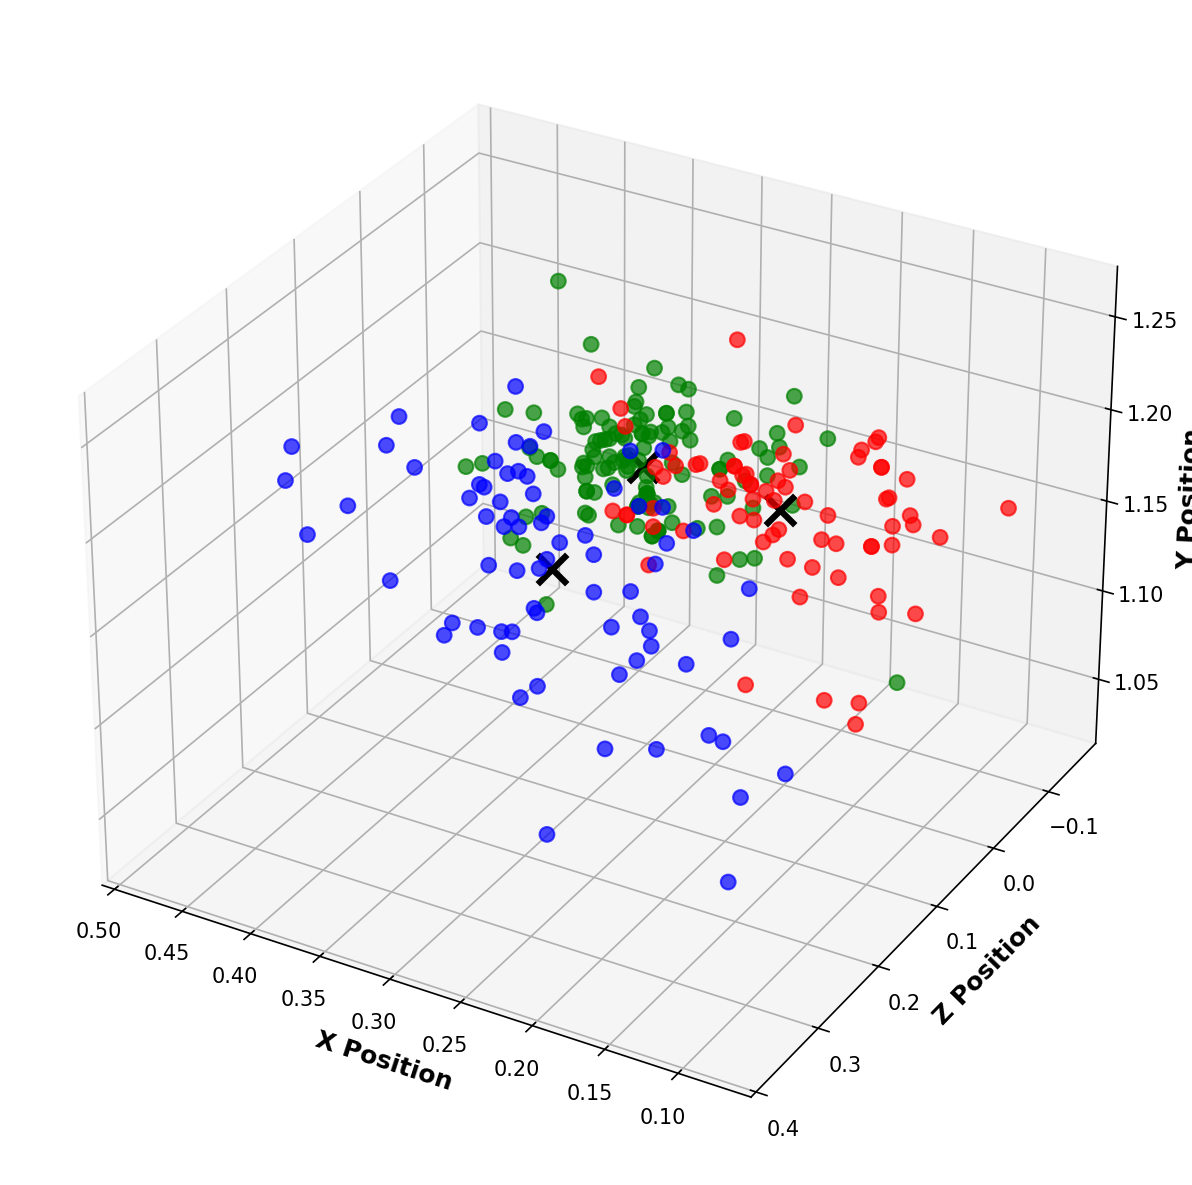
\includegraphics[width=\textwidth]{cluster_Person_1_1-A_Head_Position.png}
        \caption{Scenariul A}
    \end{subfigure}
    \hfill
    \begin{subfigure}[b]{0.32\textwidth}
        \centering
        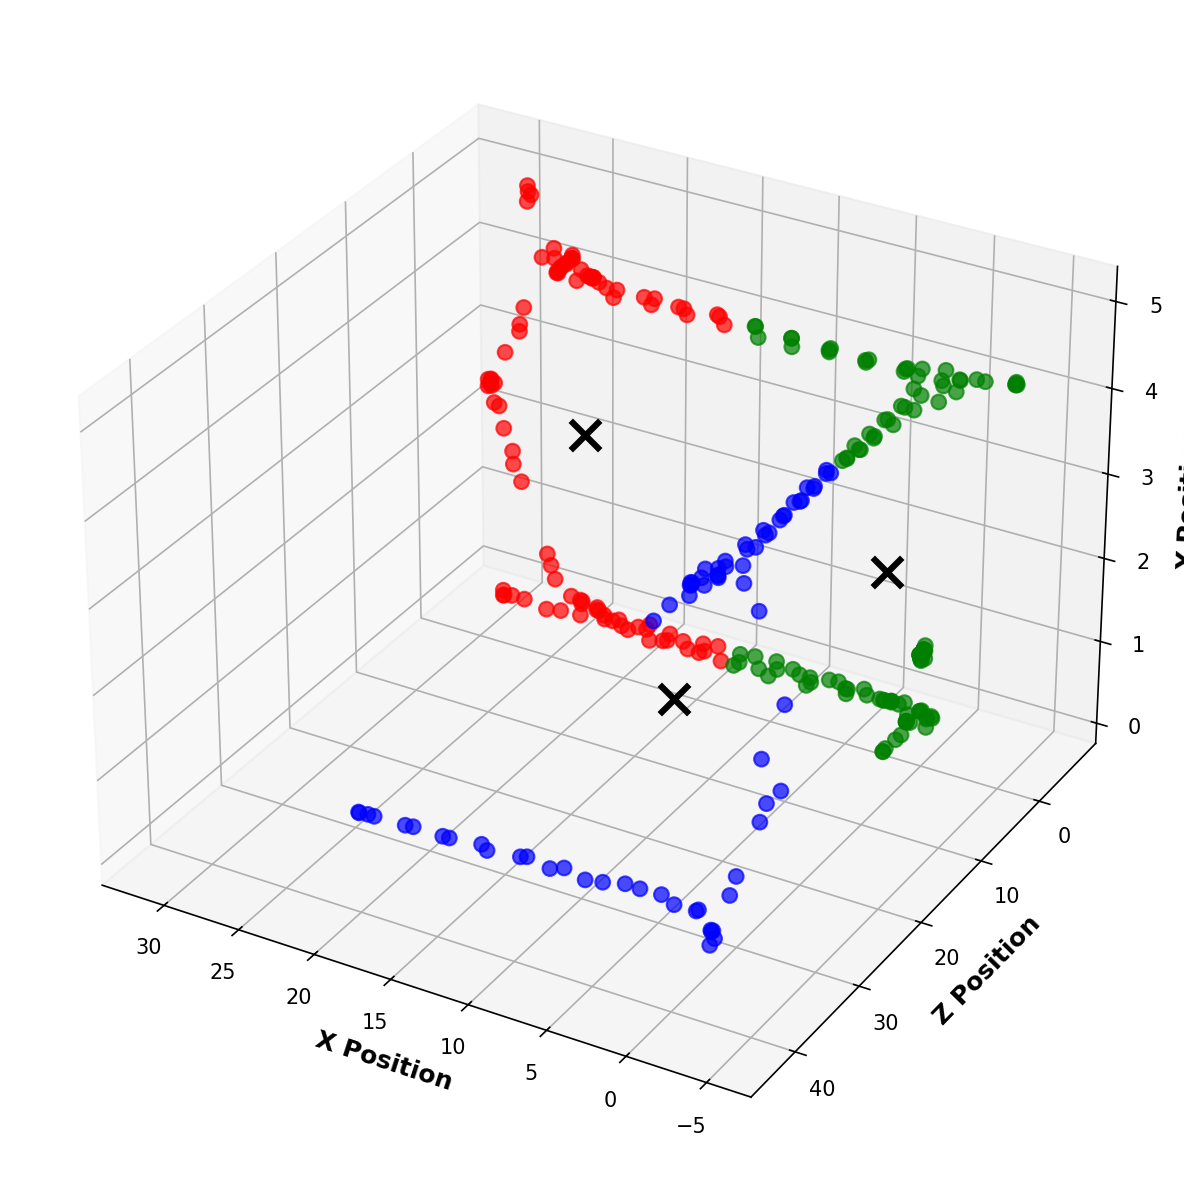
\includegraphics[width=\textwidth]{cluster_Person_1_1-B_Head_Position.png}
        \caption{Scenariul B}
    \end{subfigure}
    \hfill
    \begin{subfigure}[b]{0.32\textwidth}
        \centering
        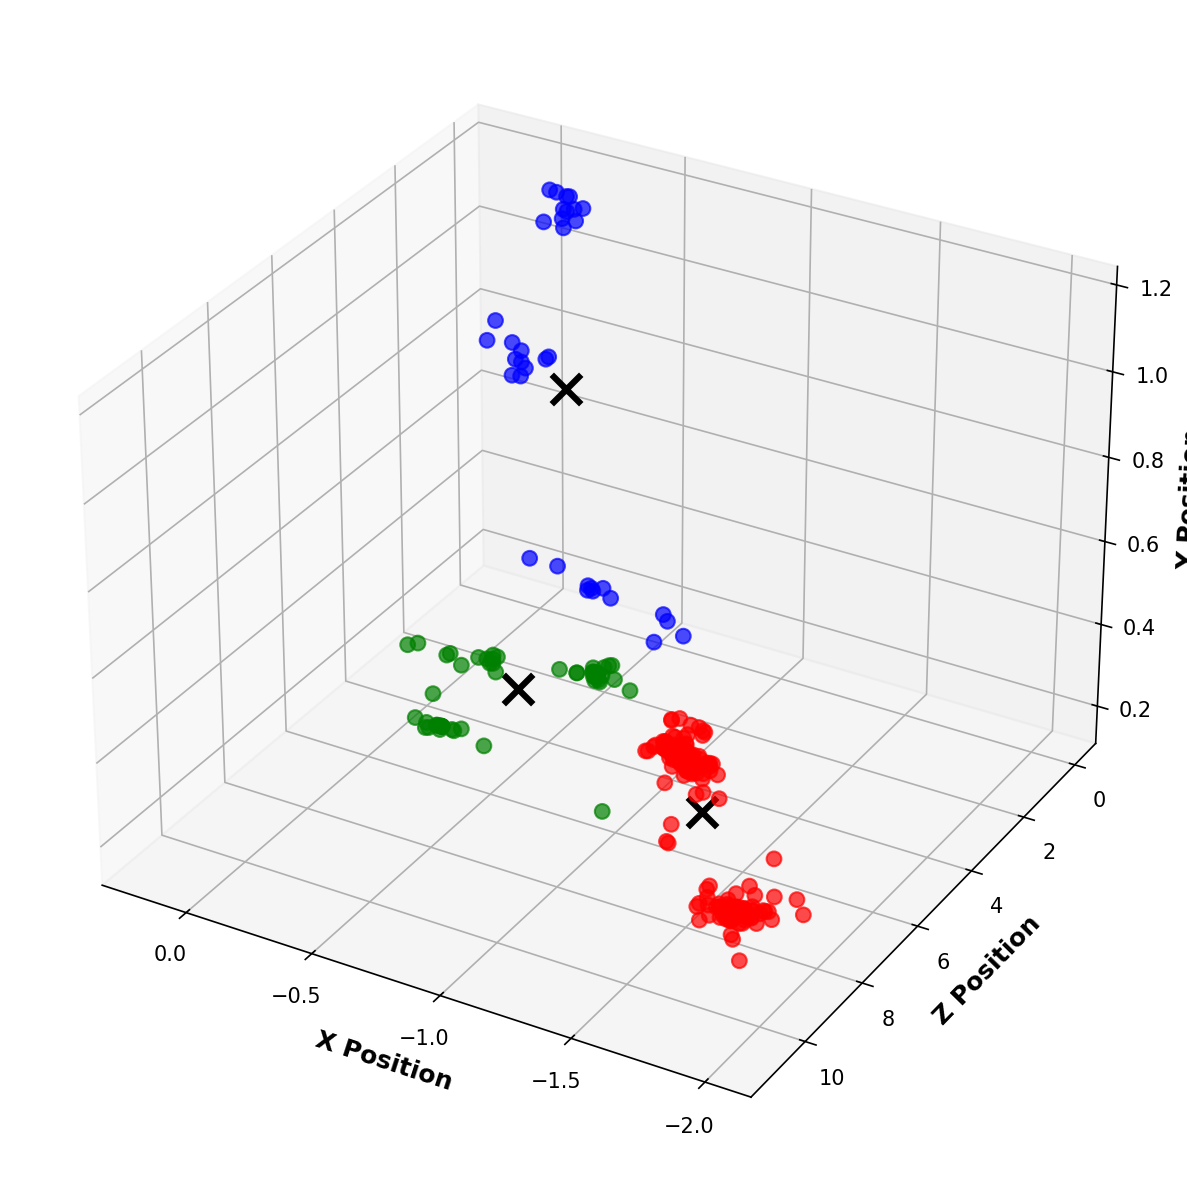
\includegraphics[width=\textwidth]{cluster_Person_1_1-C_Head_Position.png}
        \caption{Scenariul C}
    \end{subfigure}

    \caption{Comparatie scenarii VR}
\end{figure}


(4) Grafice reprezentând reconstrucția traseului parcurs de utilizator, fiecare scenariu separat

\begin{figure}[H]
    \centering

    \begin{subfigure}[b]{0.32\textwidth}
        \centering
        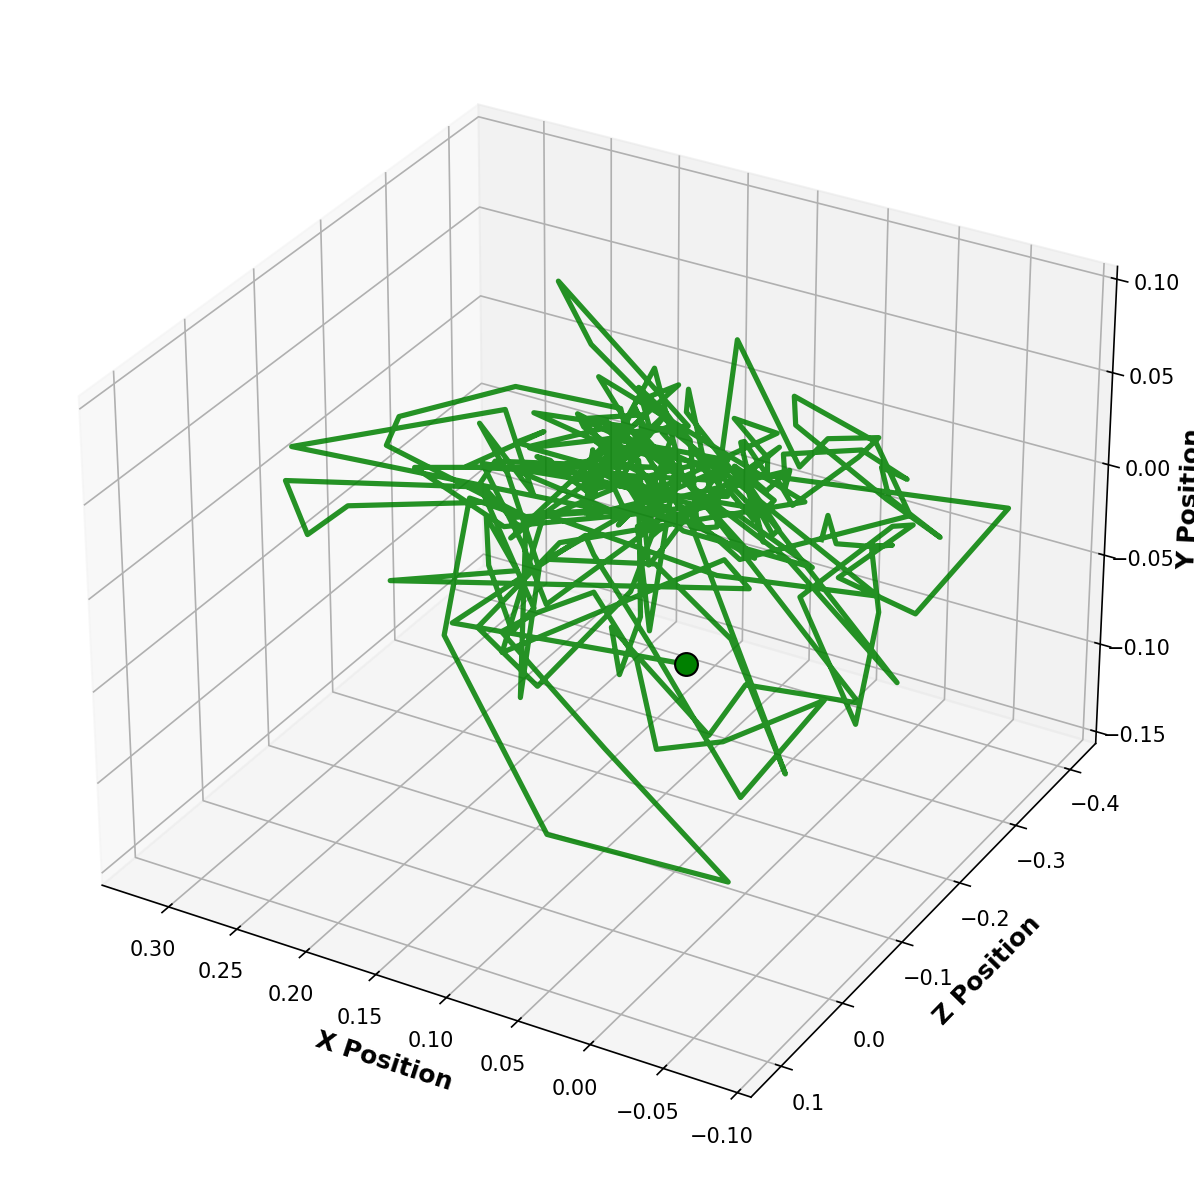
\includegraphics[width=\textwidth]{Person_1_1-A_3d_path.png}
        \caption{Scenariul A}
    \end{subfigure}
    \hfill
    \begin{subfigure}[b]{0.32\textwidth}
        \centering
        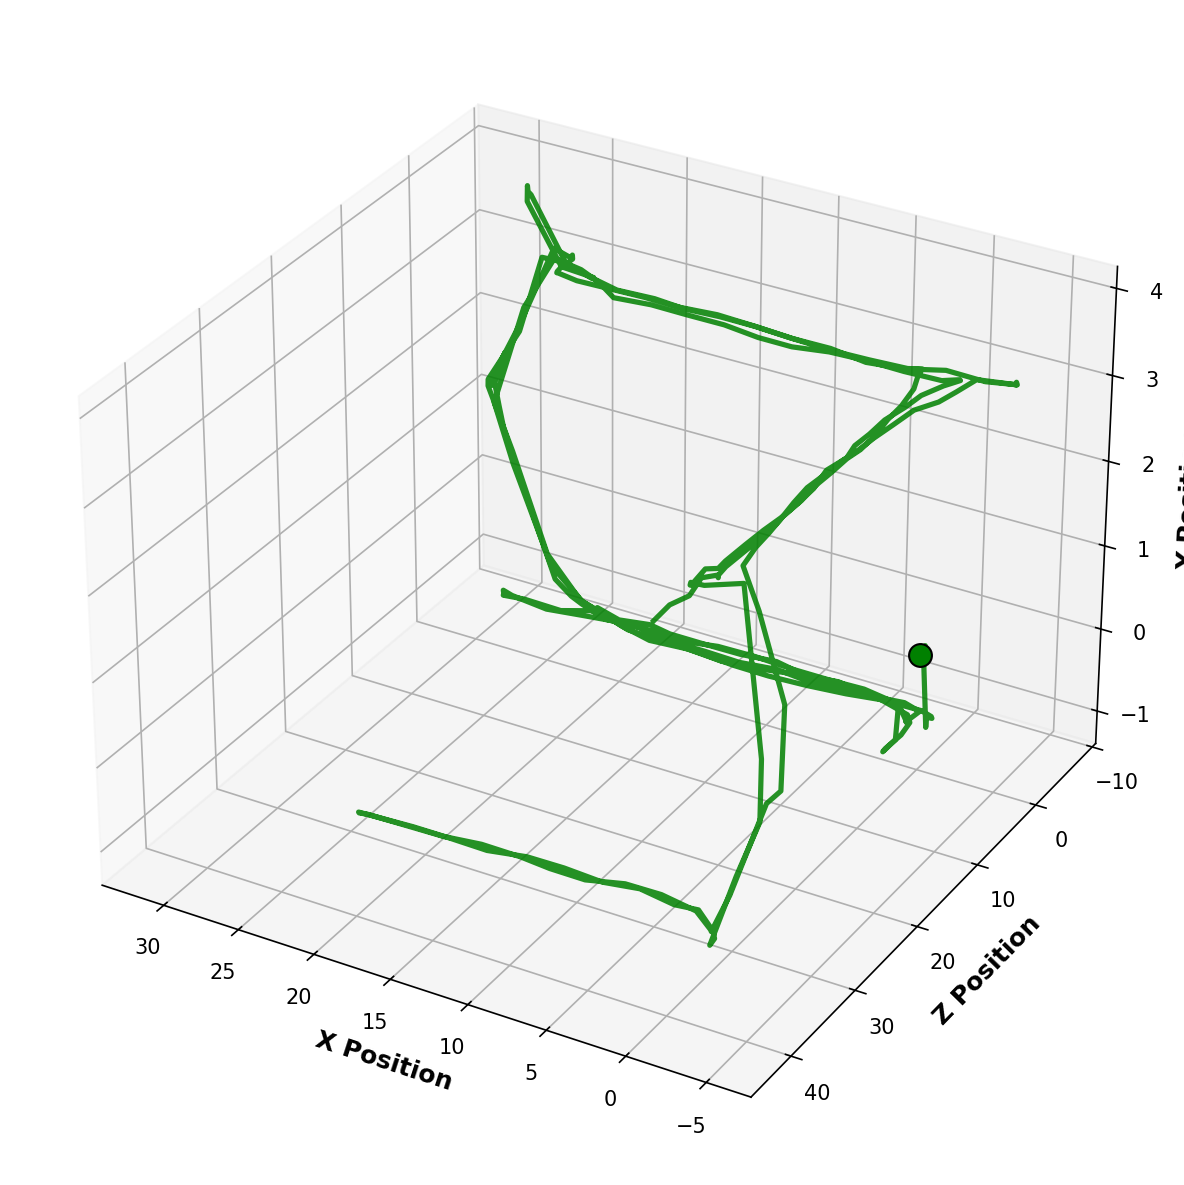
\includegraphics[width=\textwidth]{Person_1_1-B_3d_path.png}
        \caption{Scenariul B}
    \end{subfigure}
    \hfill
    \begin{subfigure}[b]{0.32\textwidth}
        \centering
        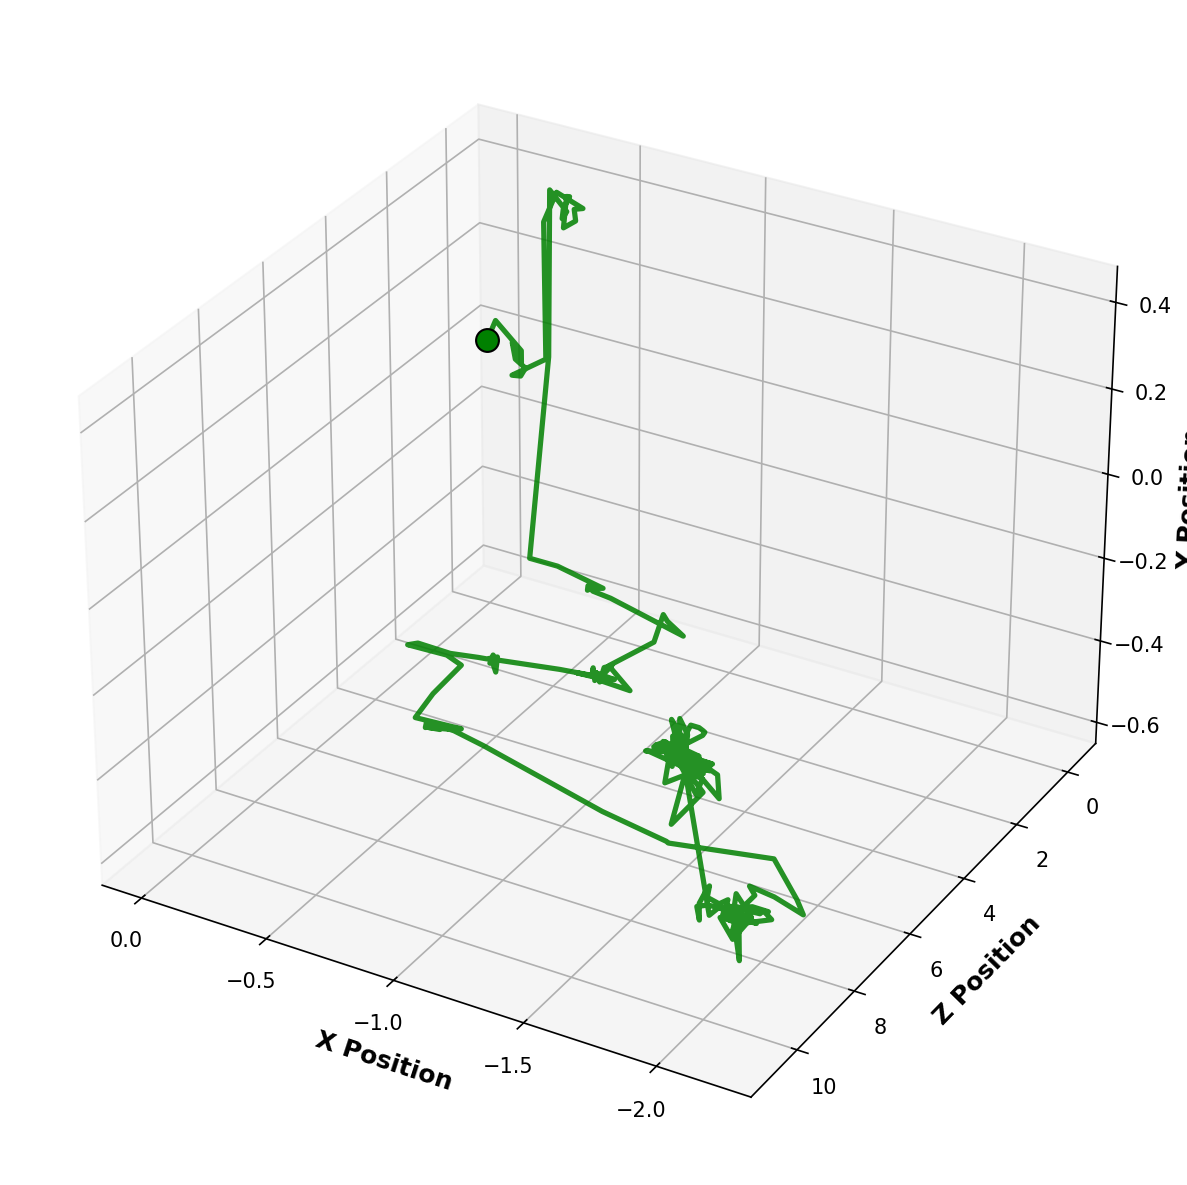
\includegraphics[width=\textwidth]{Person_1_1-C_3d_path.png}
        \caption{Scenariul C}
    \end{subfigure}

    \caption{Comparatie scenarii VR}
\end{figure}

(5) Grafice reprezentând reconstrucția traseului parcurs de utilizator, toate cele trei scenarii simultan (Vezi Figura \ref{fig:Person2}- capitolul ”Rezultate”)

(6) Grafice reprezentative pentru comparația tuturor participanților în funcție de scenariu (Vezi Figura \ref{fig:Comparatie pe scenarii} - capitolul ”Rezultate”)


Sunt generate dendrograme pentru a ilustra relațiile ierarhice și distanțele comportamentale dintre utilizatori. Gruparea este realizată prin cele două metode complementare menționate anterior. 

În plus, acest pas generează rapoarte comportamentale complete în format PDF utilizând biblioteca ReportLab, care include scorurile brute, un clasament al participanților bazat pe severitatea abaterilor și procentul total al varianței comportamentale păstrate în timpul procesului de reducere a dimensionalității, oferind astfel o imagine completă asupra fiabilității statistice a evaluării. 

\subsection{Validare}

Diagnisticele reale sunt stocate într-un fișier care este utilizat pentru a evalua și valida algoritmul. Setul de date colectat de la subiecți și cel generat de algoritm sunt aliniate. Datele sunt comparate, iar la finalul procesului, sistemul produce două docuemnte. Primul este o matrice de confuzie, al doilea este un fișier rezumat în format JSON, care consemnează acuratețea obținută, numărul total de subiecți evaluați și momentul în care s-a desfășurat evaluarea.


\chapter{Rezultate obținute}

\section{Clusterizare ierarhică aglomerativă și grupare comportamentală nesupravegheată}

Pentru interpretarea rezultatelor, au fost generate două dendrograme. Prima se bazează exclusiv pe abordarea inițială de grupare a participanților, utilizeazând cluserizarea ierarhică aglomerativă (Vezi \ref{fig:Dendrograma1}). A doua dendrogramă reprezintă o versiune optimizată, care încorporează rezultatele celei de-a doua abordări analitice. 

\begin{figure}[!ht]
    \centering
    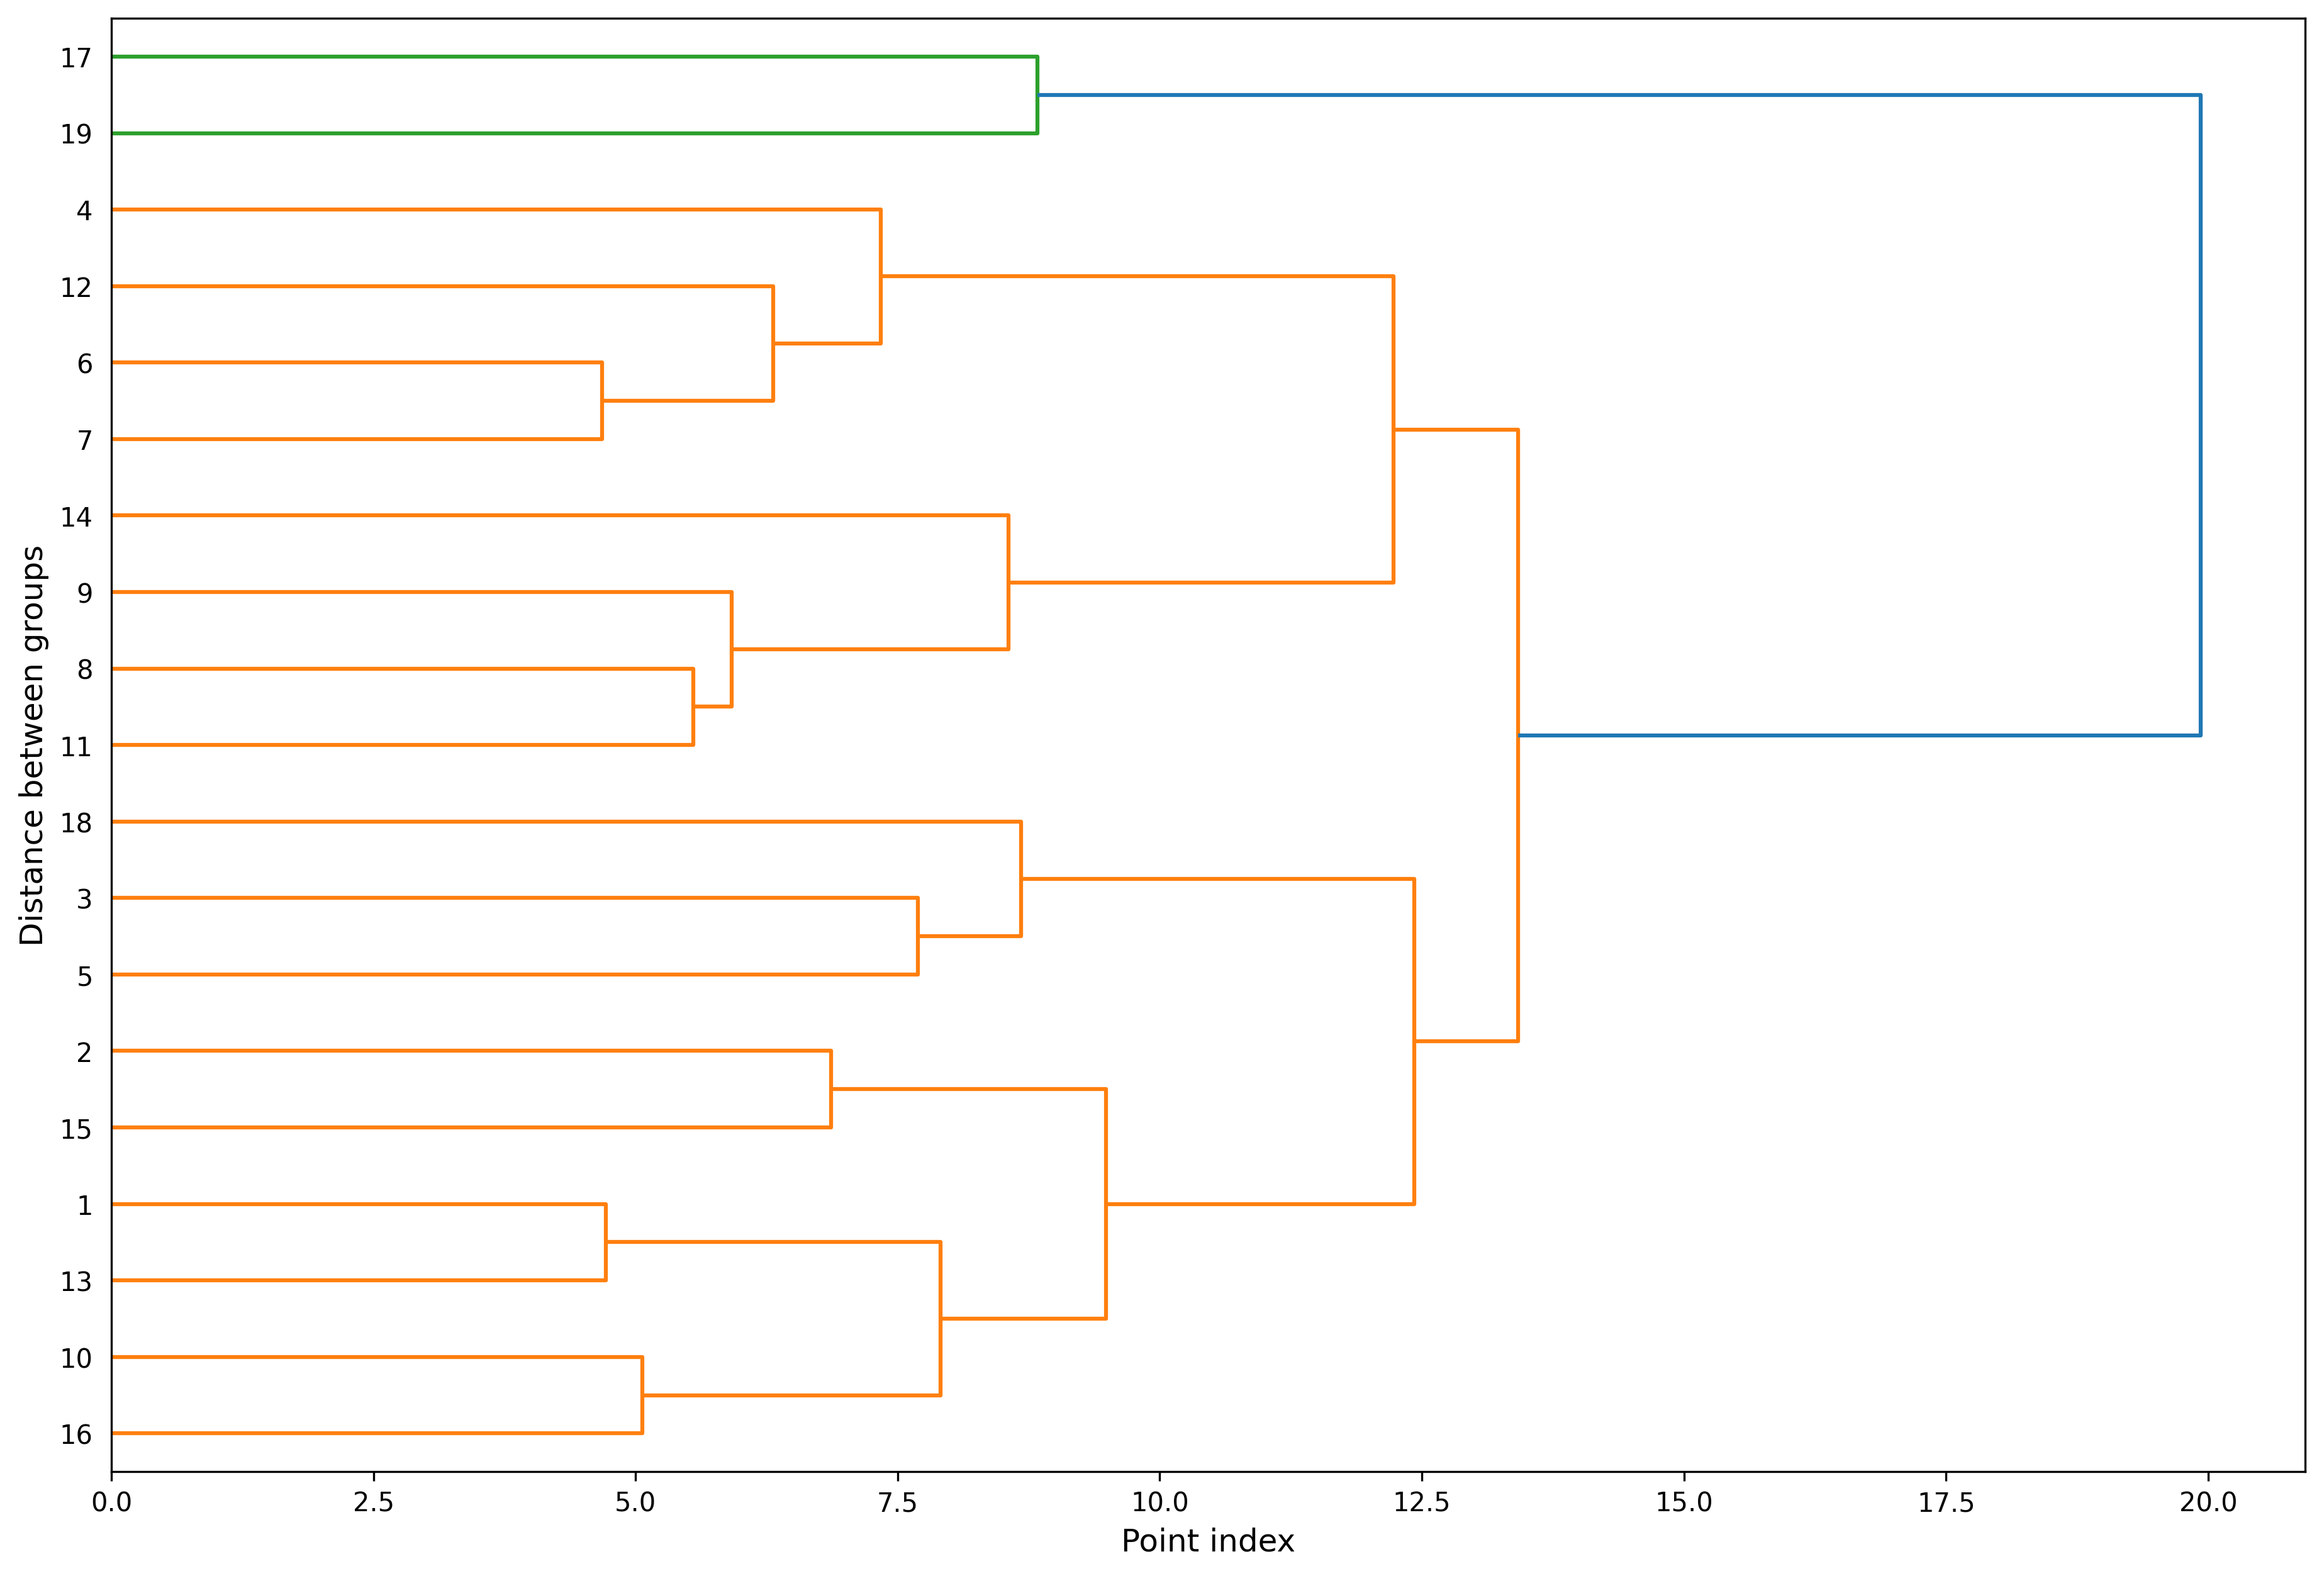
\includegraphics[width=1.0\linewidth]{dendrogram_HAC.png}
    \caption{Dendrogramă generată prin clusterizare ierarhică aglomerativă.}
    \label{fig:Dendrograma1}
\end{figure}

Dendrograma inițială ilustrează similaritățile dintre participanți; cu toate acestea, oferă o perspectivă limitată asupra naturii acestor similarități, furnizând doar o vizualizare preliminară a comportamentelor analizate. Pe axa verticală (stânga), sunt reprezentați participanții individuali, în timp ce axa orizontală (jos) mapează distanțele dintre punctele de date. O analiză mai precisă și mai relevantă este reflectată începând cu Figura \ref{fig:Dendrograma2}. 

Această dendrogramă optimizată oferă o perspectivă mai profundă, reflectând nu doar grupările comportamentale, ci și modul în care abordarea și datele îmbunătățite interpretează informațiile. În consecință, în acest grafic pot fi observate grupări distincte față de cel anterior. În acest caz, apar două clustere principale: un grup semnificativ format din 17 participanți și un grup minoritar format din 2 participanți, acesta din urmă reprezentând un tipar comportamental distinct. Bara verticală din stânga ilustrează distanța dintre puncte. O distanță de aproximativ 20 indică o divergență semnificativă între cele două grupuri.

Anumiți participanți prezintă comportamente foarte similare (de exemplu, Person\_12, Person\_2, Person\_14, Person\_15), indicând o similaritate intragrup ridicată, fără anomalii care ar necesita intervenții detaliate imediate. În cadrul grupului marcat cu verde, sunt identificați 17 participanți.
Ultimii trei subiecți din acest subgrup sunt clasificați corect ca făcând parte din grupul persoanelor cu dizabilități motorii. Tiparele comportamentale ale primilor trei subiecți din acest grup vor fi analizate în detaliu în subsecțiunile următoare pentru a justifica această clasificare.

Existența acestor două grupuri distincte, în special a grupului minoritar, face ca o analiză detaliată să fie atât utilă, cât și necesară pentru acest studiu.

\begin{figure}[!ht]
    \centering
    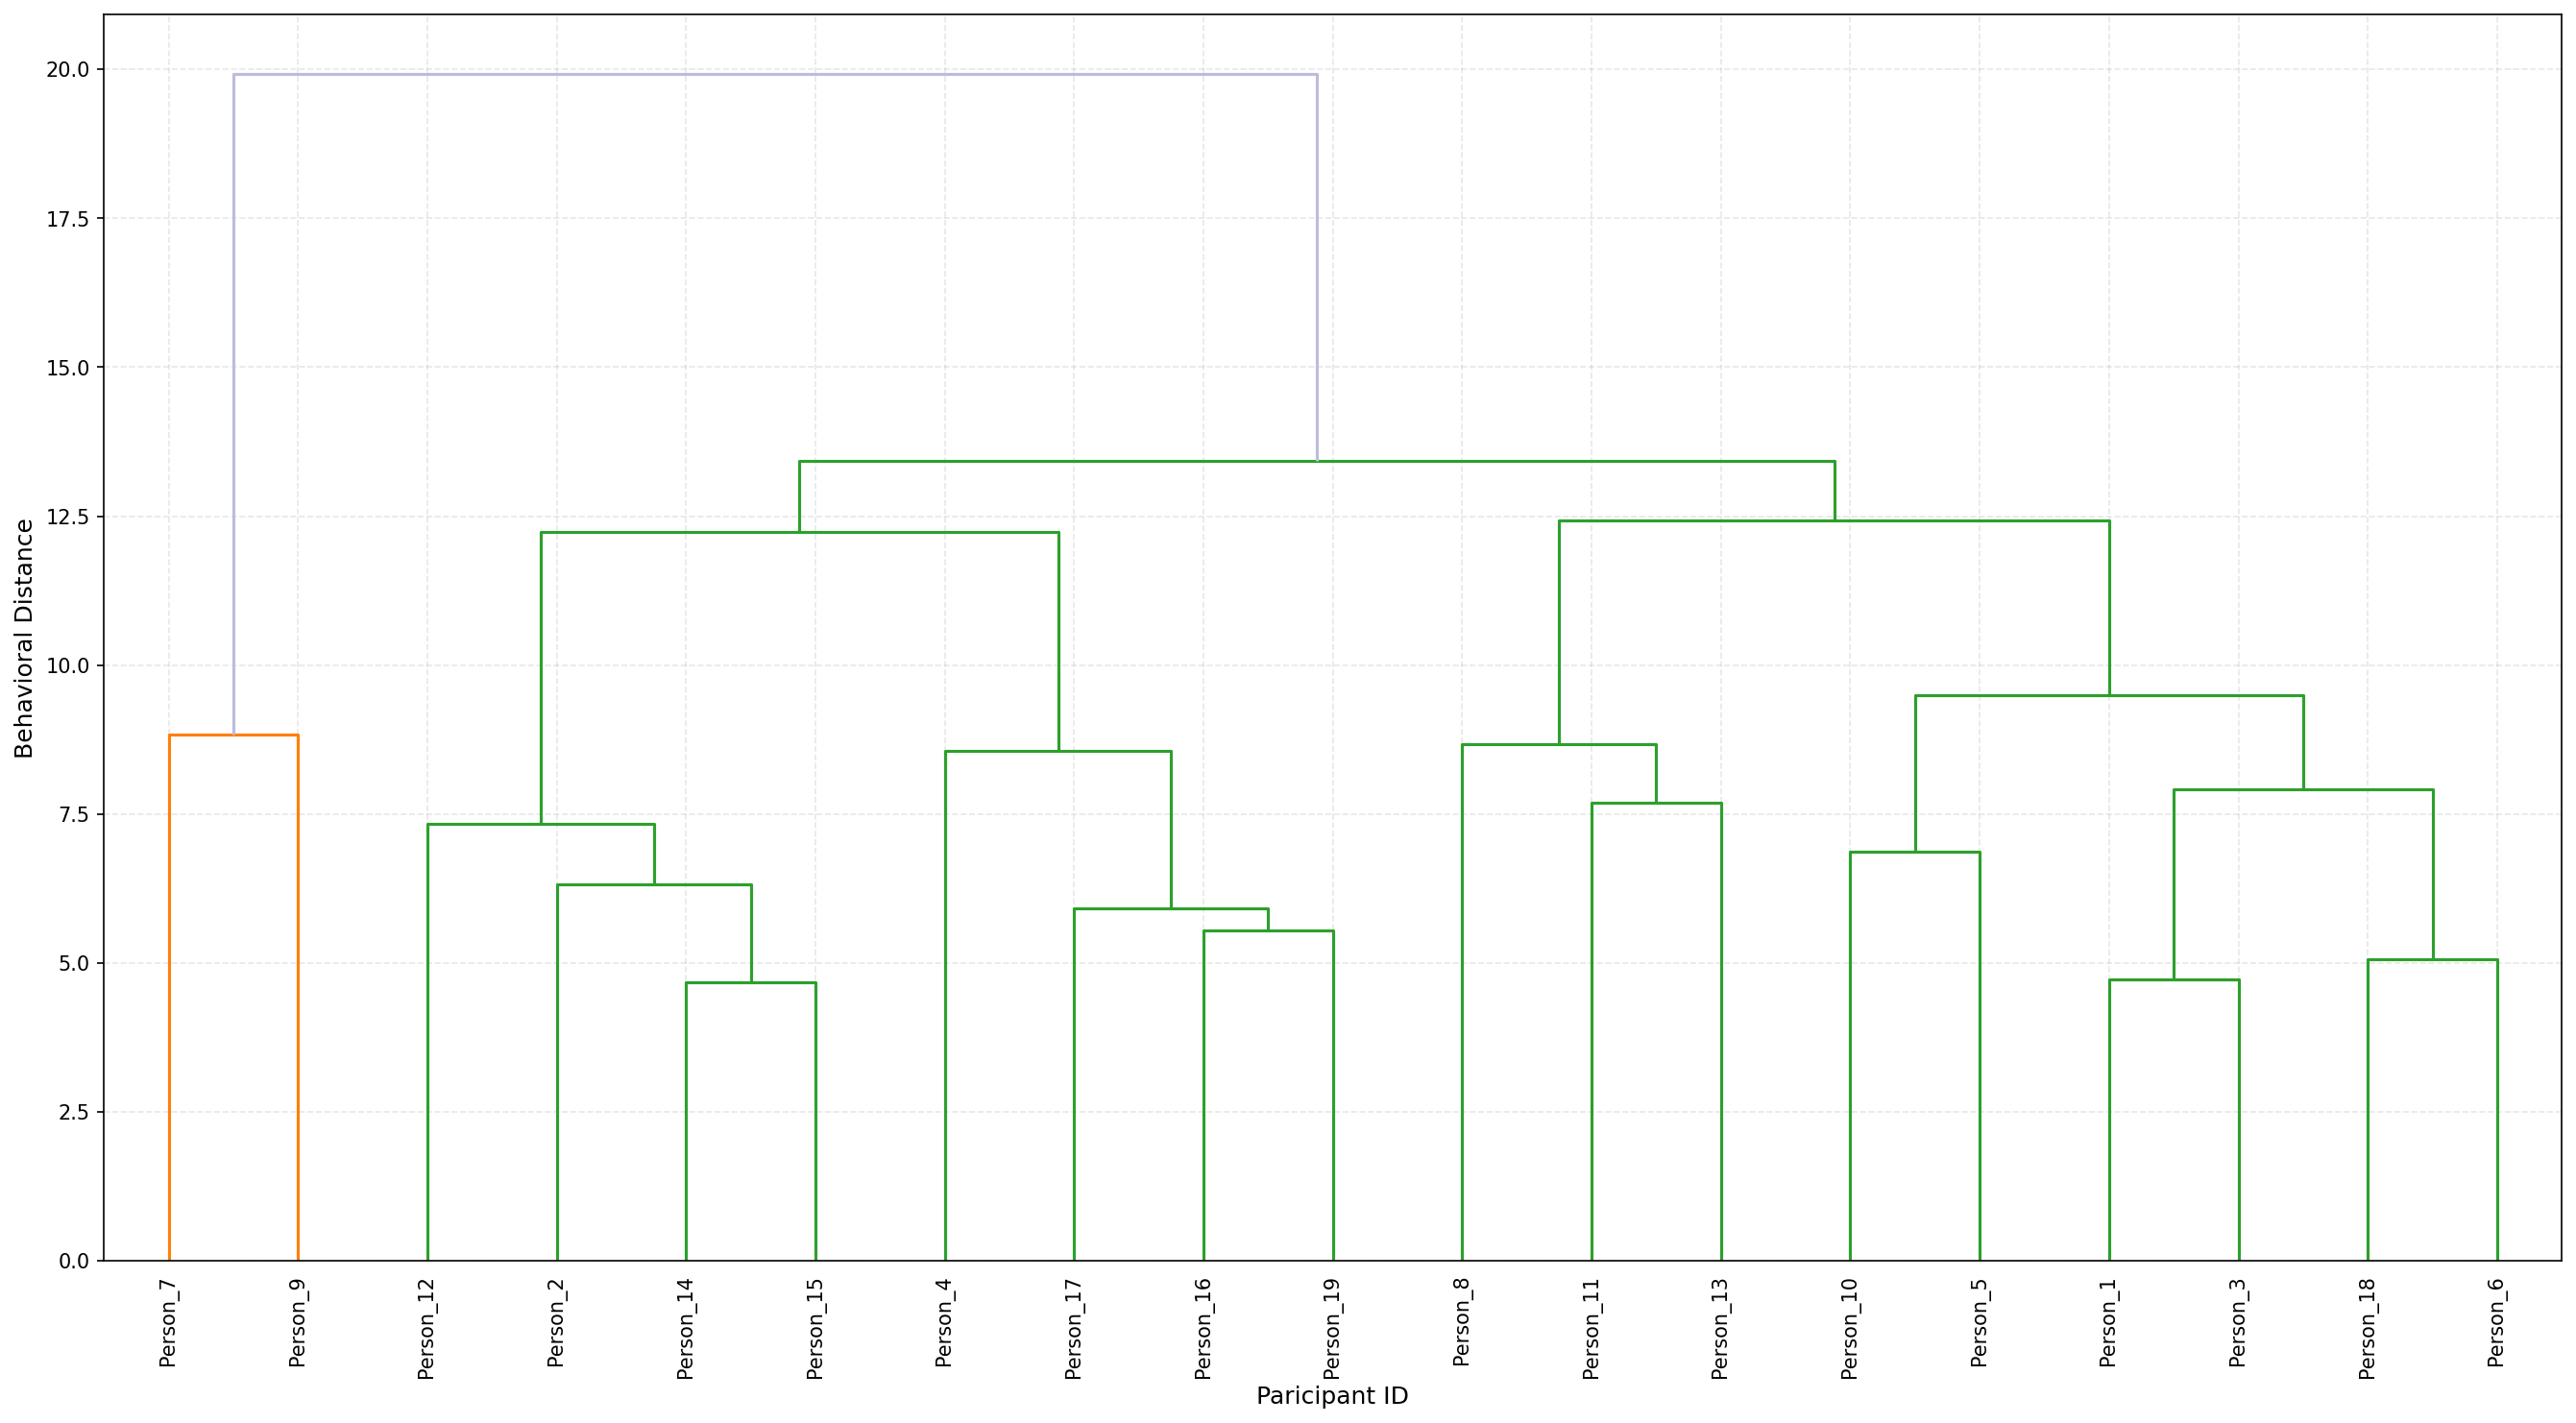
\includegraphics[width=0.8\linewidth]{participant_similarity_dendrogram.png}
    \caption{Dendrogramă rafinată a similarității participanților, bazată pe a doua metodă de grupare.}
    \label{fig:Dendrograma2}
\end{figure}

\section{Profile de bază ale participanților}
Setul de date colectat de la participanți include cinci persoane cu dizabilități. Datele de mișcare ale acestor subiecți sunt identificate în cadrul studiului sub denumirile: „Person\_4”, „Person\_5”, „Person\_7”, „Person\_9” și „Person\_11”. Acești participanți sunt de interes deosebit pe parcursul fazei de analiză.

\section{Analiză calitativă}

Pe baza graficelor generate, patru participanți au fost selectați ca studii de caz reprezentative, deoarece evidențiază cel mai bine diferențele comportamentale relevante pentru problema investigată. Primul subiect, identificat ca Person\_2 (Vezi \ref{fig:Person2}), servește drept referință pentru comportamentul normativ conform analizei. 

\begin{figure}
    \centering
    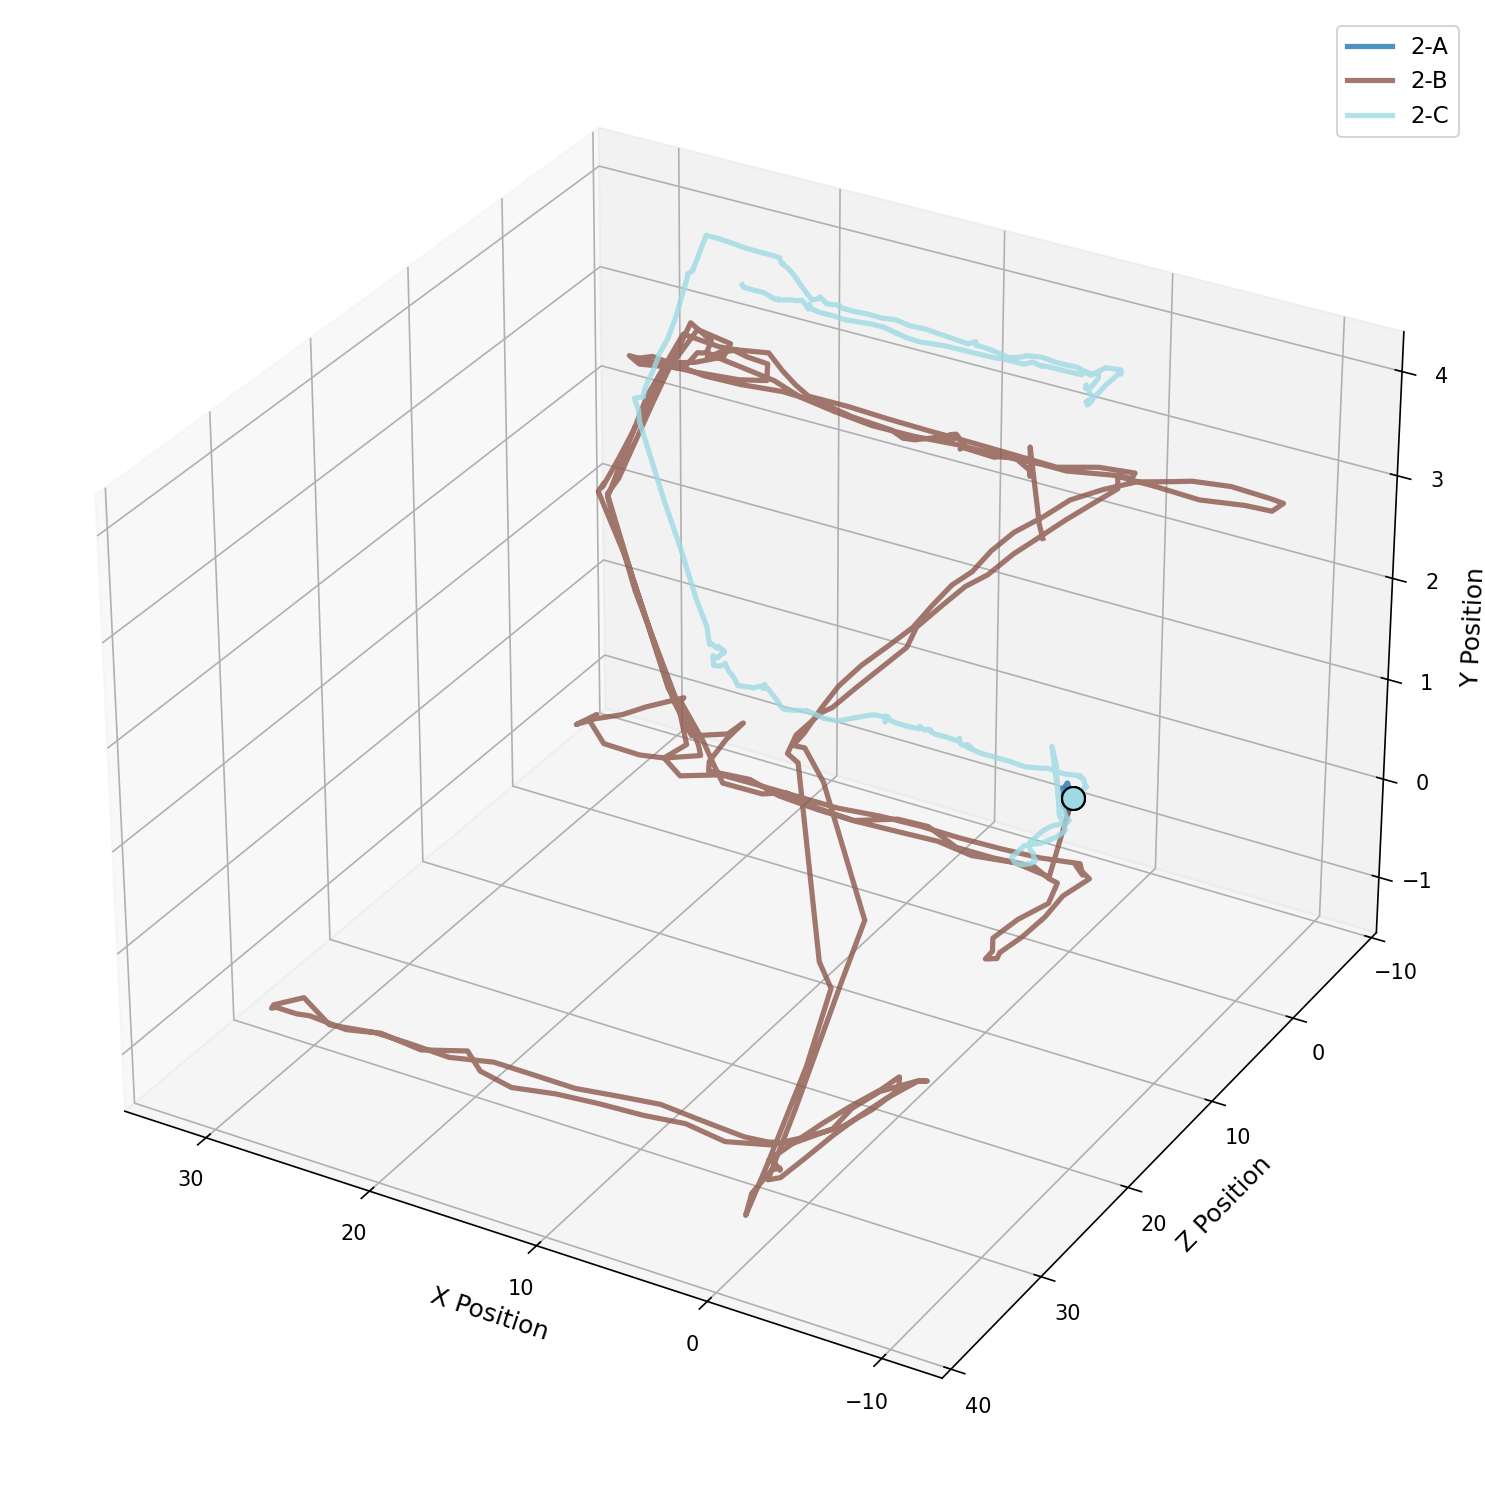
\includegraphics[width=0.5\linewidth]{Person_2_scenarios_comparison.png}
    \caption{Vizualizare comparativă a distribuției spațiale și a clusterelor de mișcare pentru Person\_2 în Scenariile A, B și C.}
    \label{fig:Person2}
\end{figure}

Acesta prezintă un tipar de mișcare echilibrat și bine organizat în toate cele trei etape. În Scenariul A, deși este necesară menținerea poziției staționare, clusterele indică rotații active ale capului, ceea ce semnalează un nivel ridicat de atenție și explorare a mediului. În Scenariul B, echilibrul aproape perfect între zone și traseele de navigație clare indică o înțelegere sistematică a mecanicii complexe. 
Acesta prezintă un tipar de mișcare echilibrat și bine organizat în toate cele trei etape. În Scenariul A, deși este necesară menținerea poziției staționare, clusterele indică rotații active ale capului, ceea ce semnalează un nivel ridicat de atenție și explorare a mediului.  În Scenariul C, echilibrul aproape perfect între zone și traseele de navigație clare indică o înțelegere sistematică a mecanicii complexe. 

Pentru a evidenția deviațiile de la această linie de bază, ceilalți trei subiecți (Vezi Figura \ref{fig:Comparatie subiecti atipici}) prezintă profile atipice.

Person\_4 afișează un comportament atipic comparativ cu Person\_2, în principal din cauza nivelului inconsistent de explorare și implicare între scenarii. În Scenariul A, deși sarcina impunea menținerea poziției staționare, Person\_4 nu a prezentat aproape nicio mișcare a capului (94.4\% dintre puncte fiind încadrate într-un singur cluster), contrastând puternic cu scanarea activă a capului și clusterele bine separate ale persoanei Person\_2. În Scenariul C, mișcarea persoanei Person\_4 rămâne relativ restricționată și localizată, în timp ce Person\_2 explorează întreg spațiul într-un mod echilibrat. Prin urmare, deși performanța în Scenariul B este una bună, lipsa explorării în Scenariul A și restricțiile spațiale din Scenariul C sugerează un profil instabil și atipic.

În continuare, Person\_7 prezintă un comportament puternic atipic. Spre deosebire de Person\_2, care explorează mediul atât pe plan vertical, cât și orizontal, Person\_7 rămâne aproape exclusiv într-un singur plan orizontal, indicând o limitare clară pe axa Y (fără a depăși valoarea de +3 chiar și în scenariul liber C). În Scenariul B, unde mecanica necesită activarea privirii în sus, Person\_7 nu utilizează această strategie, rămânând în proporție de 91.4\% staționar într-o zonă mică. Acest lucru sugerează o incapacitate de a efectua mișcări verticale ale capului. Astfel, în contrast cu profilul sănătos și adaptiv al persoanei Person\_2, Person\_7 reprezintă o anomalie extremă caracterizată prin lipsa explorării verticale și incapacitate de adaptare la navigarea bazată pe privire.

Person\_9 prezintă de asemenea un profil puternic atipic, diferind semnificativ de Person\_2 atât în direcția mișcării, cât și în interacțiunea cu mediul. În timp ce Person\_2 menține o postură echilibrată și utilizează corect atât planul orizontal, cât și pe cel vertical, Person\_9 prezintă o orientare persistent descendentă (valori negative pe axa Y în toate etapele) și nu reușește să acceseze zonele superioare de mișcare necesare în Scenariul B. În loc să navigheze liber și organizat, precum Person\_2, Person\_9 rămâne restricționat la nivelul solului, prezentând mișcare fragmentată în Scenariul B și o restricție extremă de explorare în Scenariul C, unde subiectul devine aproape static. Person\_9 evidențiază un tipar persistent de orientare descendentă și restricție spațială severă, marcând un caz clar atipic.

\begin{figure}[H]
    \centering
    
    \begin{minipage}{0.32\textwidth}
        \centering
        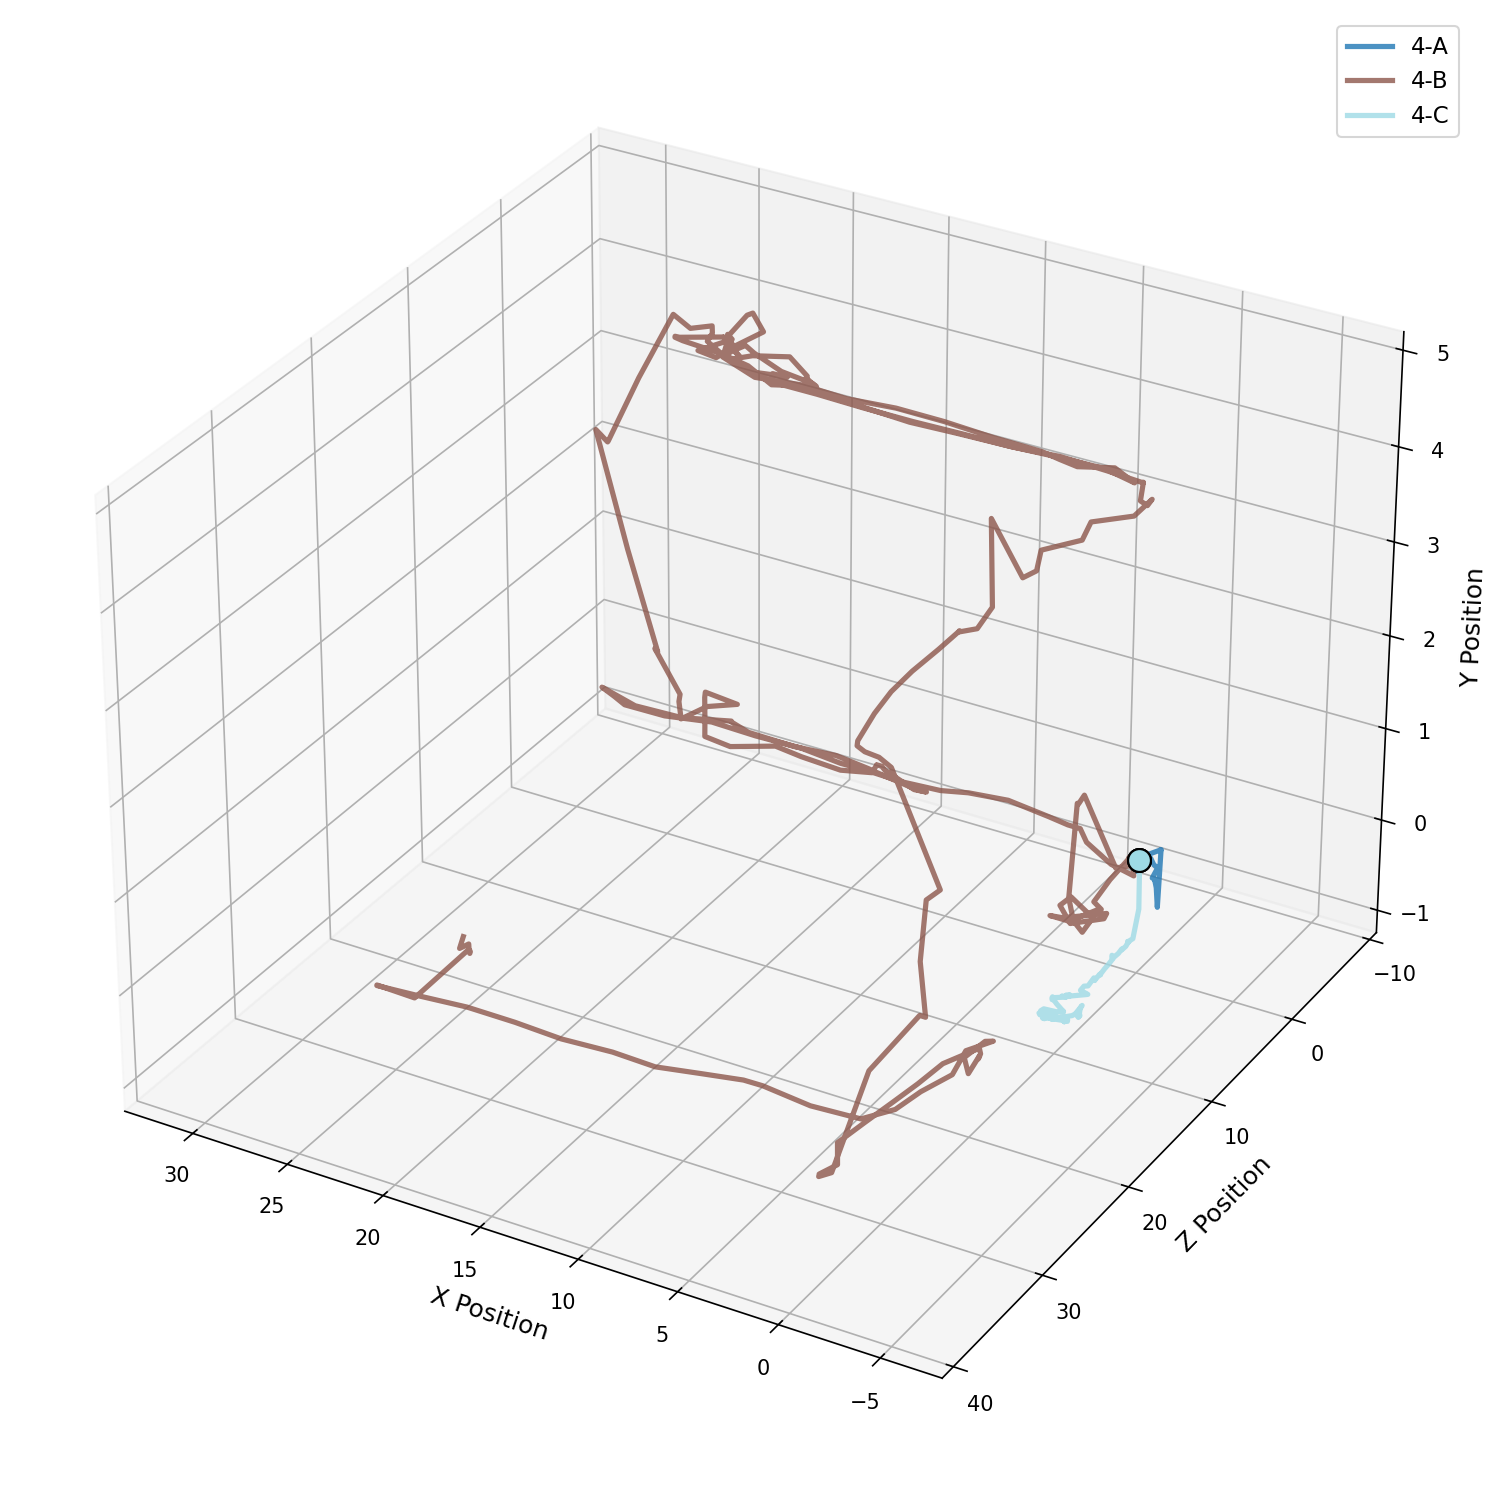
\includegraphics[width=\textwidth]{Person_4_scenarios_comparison.png}
        \caption{Person\_4}
    \end{minipage}
    \hfill
    \begin{minipage}{0.32\textwidth}
        \centering
        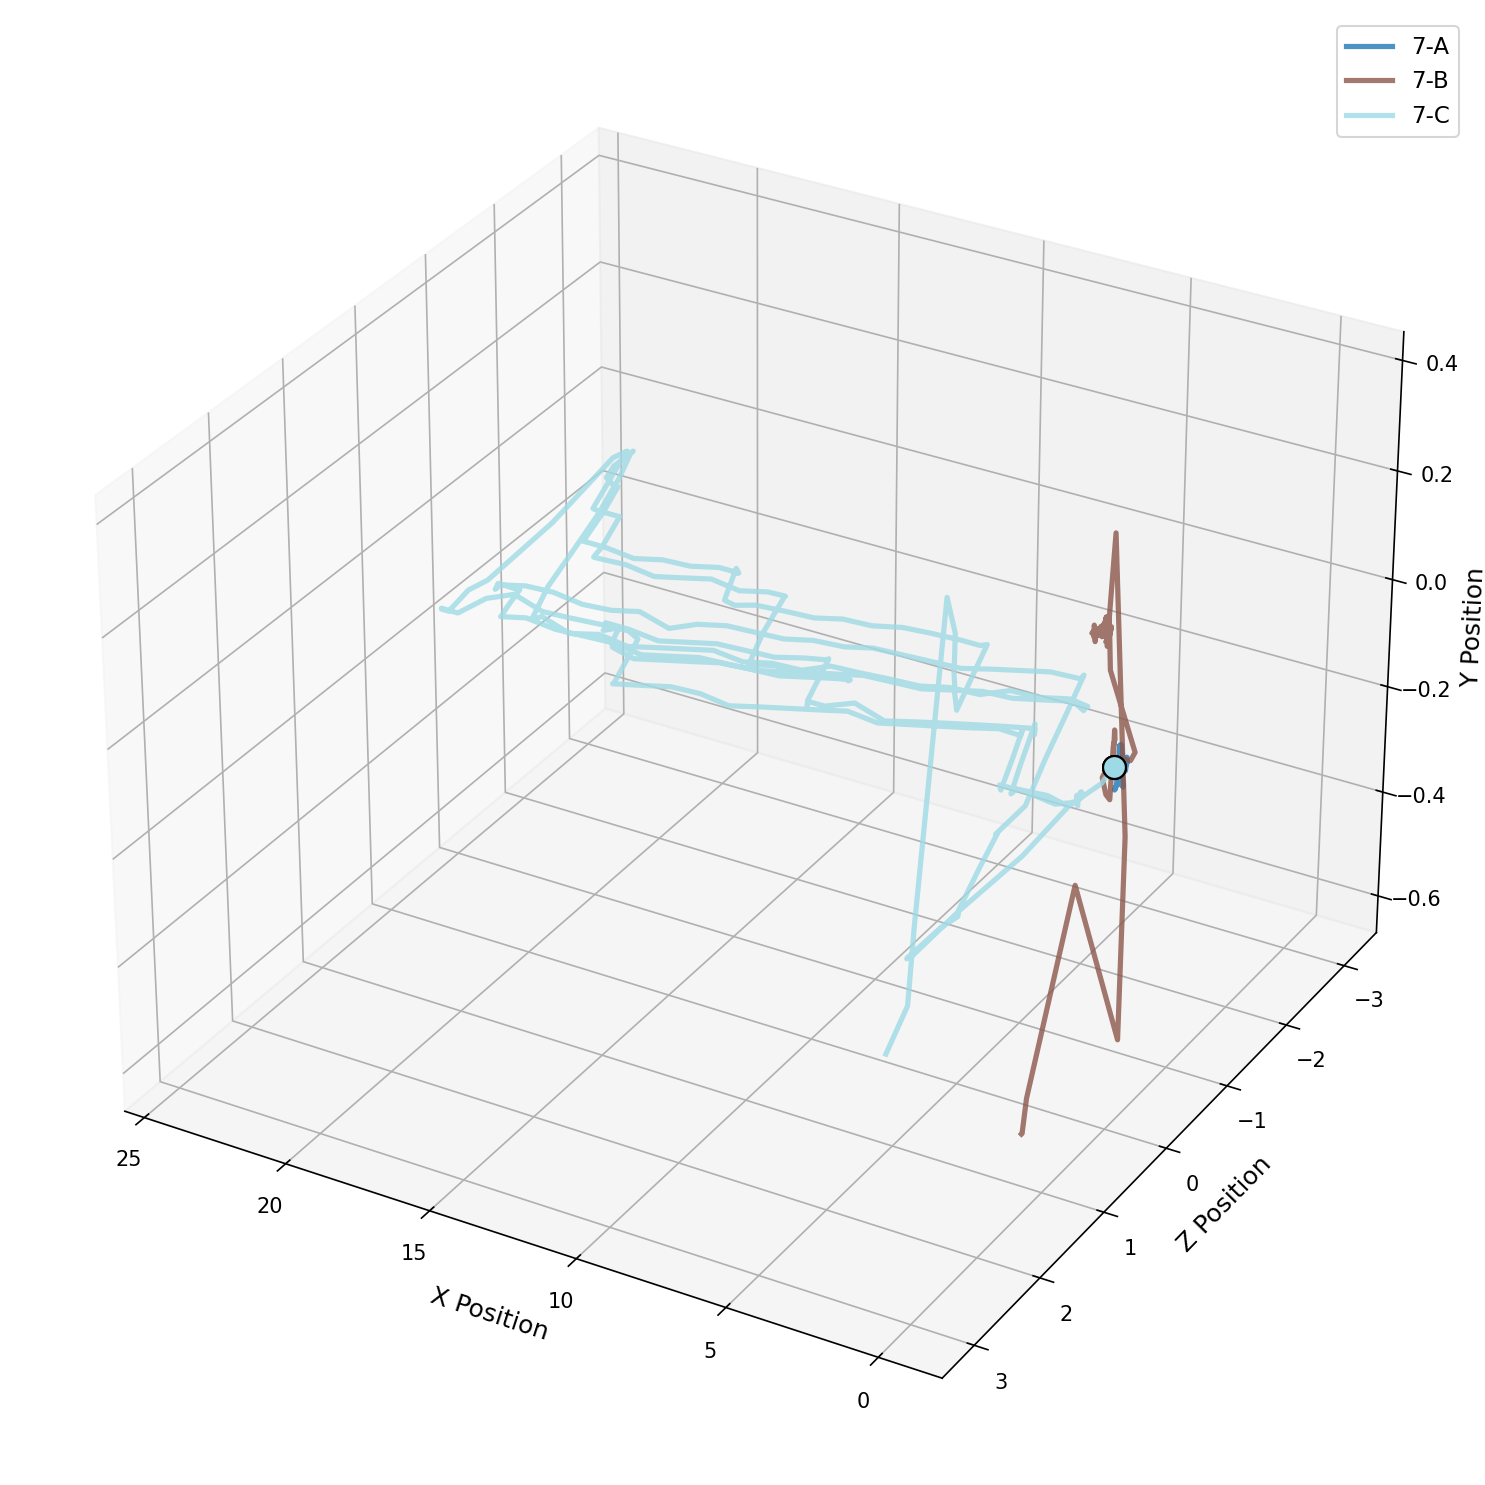
\includegraphics[width=\textwidth]{Person_7_scenarios_comparison.png}
        \caption{Person\_7}
    \end{minipage}
    \hfill
    \begin{minipage}{0.32\textwidth}
        \centering
        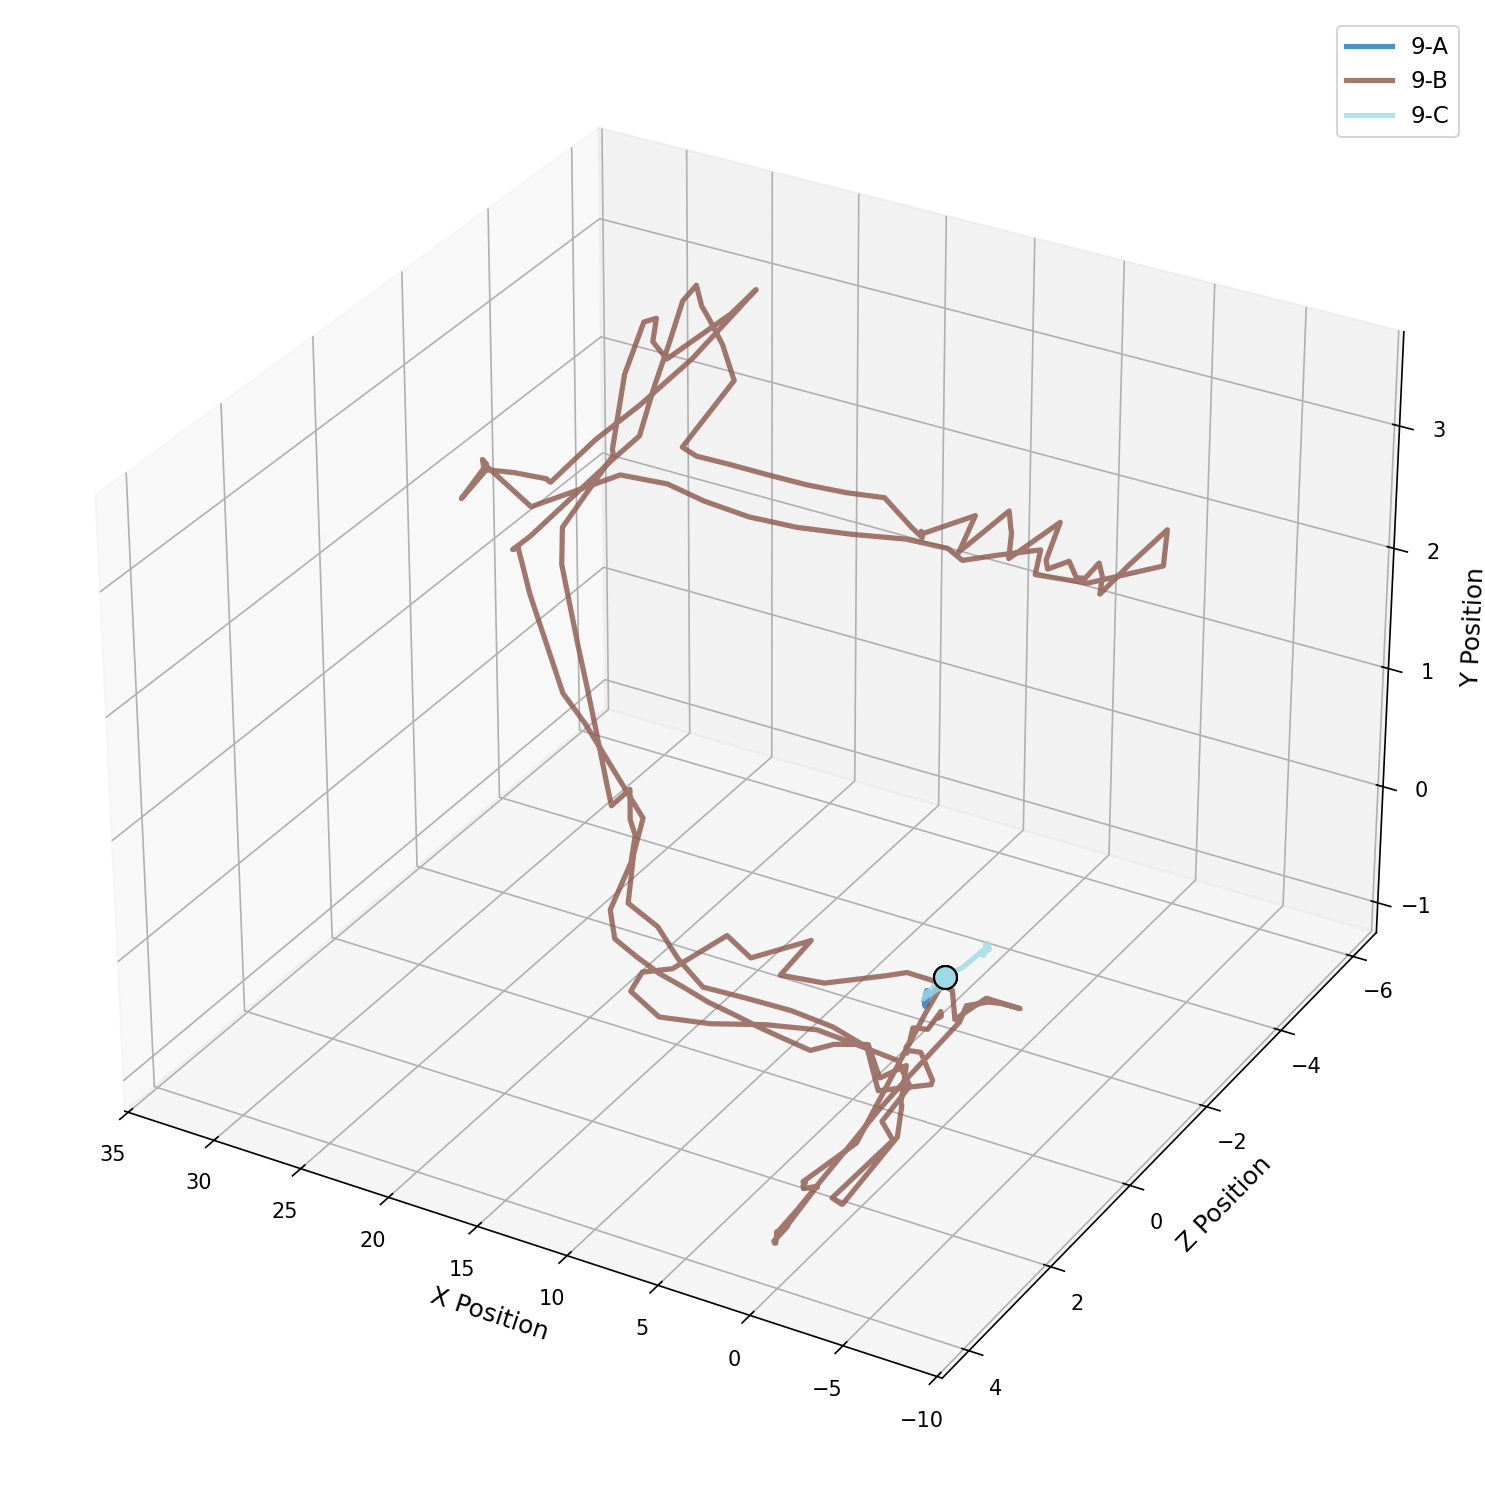
\includegraphics[width=\textwidth]{Person_9_scenarios_comparison.png}
        \caption*{Person\_9}
    \end{minipage}

    \caption{Reprezentare vizuală comparativă a distribuției spațiale și a clusterelor de mișcare pentru Persoana\_4, Persoana\_7 și Persoana\_9 în Scenariile A, B și C.}
    \label{fig:Comparatie subiecti atipici}
\end{figure}

În plus, Person\_11 (Vezi Figura \ref{fig:Person11}) prezintă un profil distinct care, în ciuda intensității sale, servește drept exemplu de atipicitate. Person\_11 manifestă un nivel excesiv și fragmentat de explorare spațială, sugerând mai degrabă hiperactivitate motorie decât eficiență funcțională. În Scenariul B, acest tip de navigare generează tipare de mișcare inconsistente, care contrastează cu comportamentul controlat al grupului de bază. În consecință, acoperirea 3D extinsă și variațiile verticale spontane ale lui Person\_11 sunt clasificate ca indicatori ai instabilității comportamentale.

\begin{figure}[H]
    \centering
    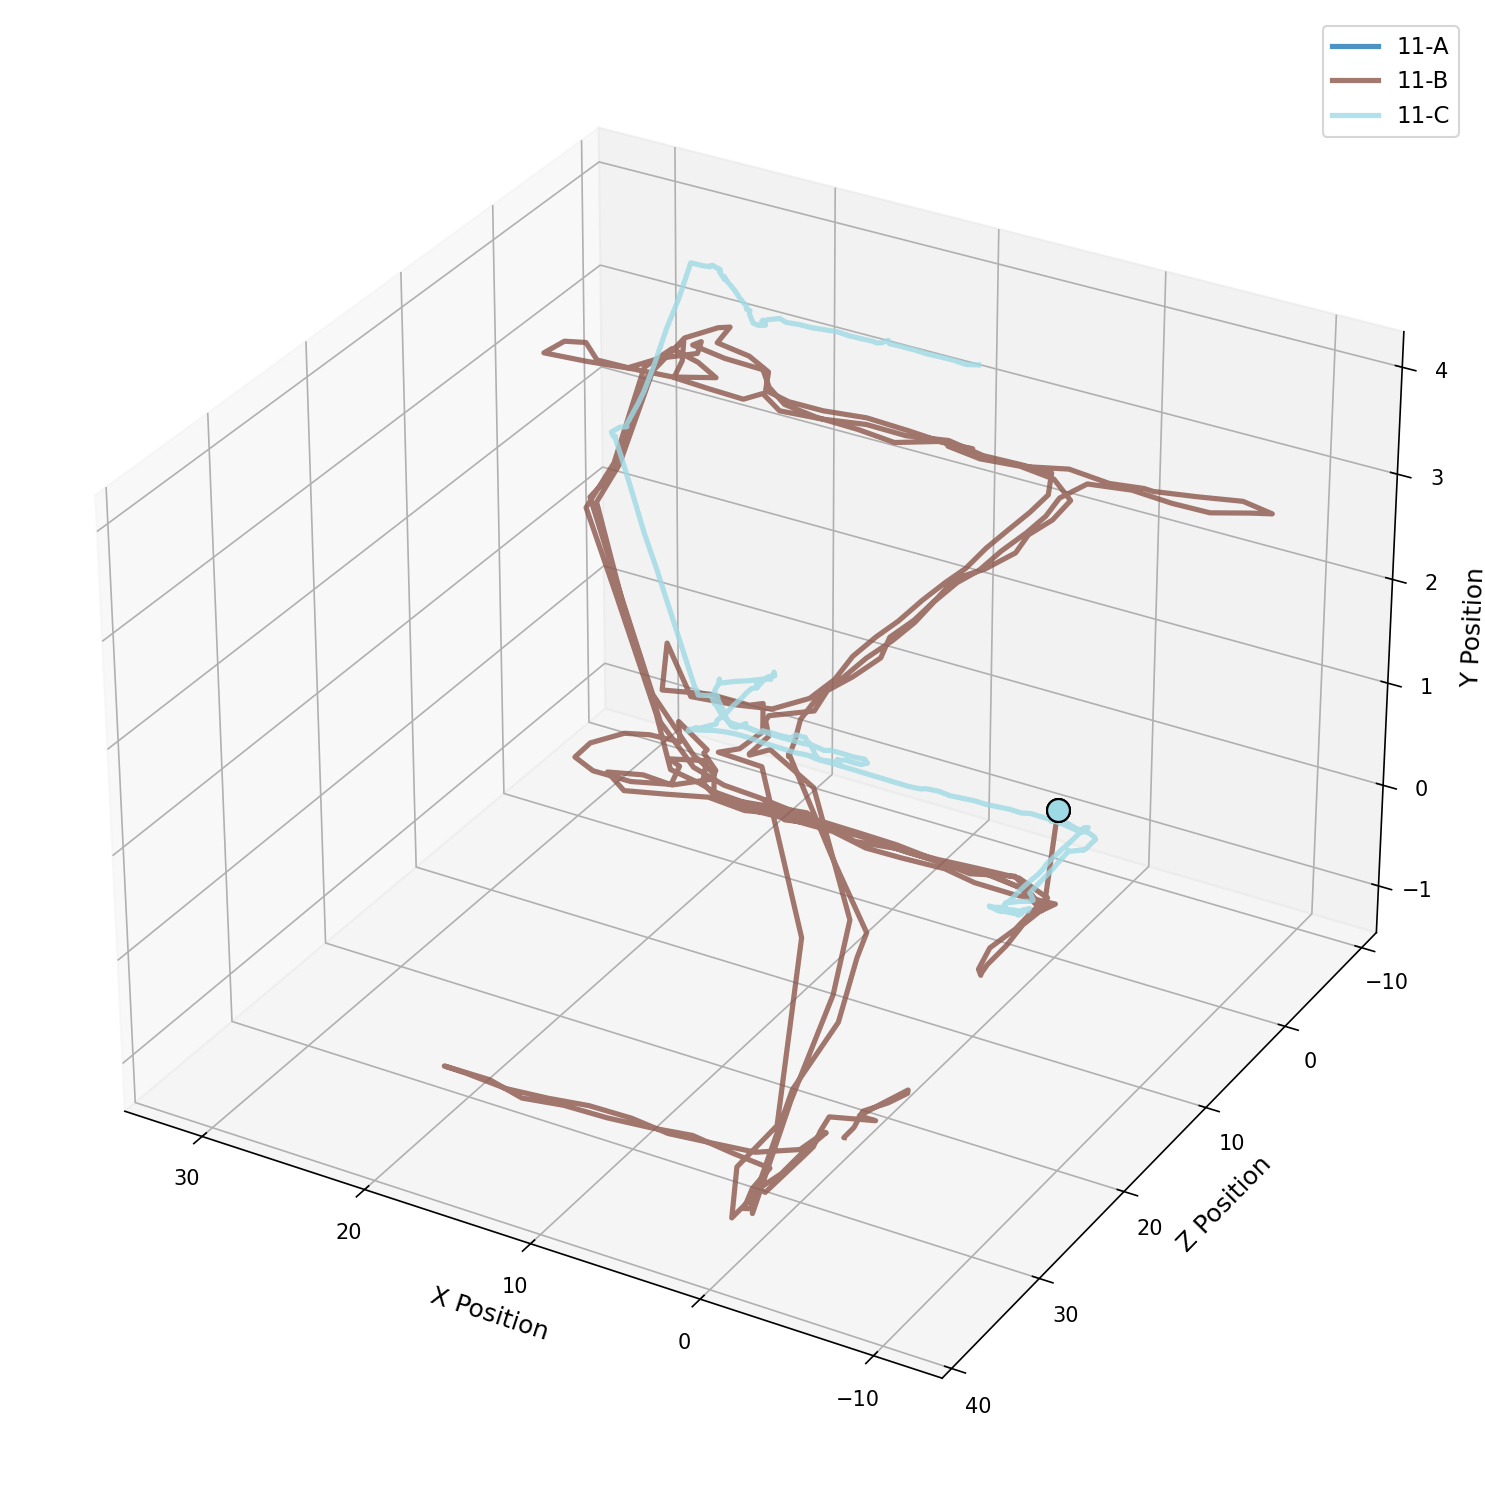
\includegraphics[width=0.5\linewidth]{Person_11_scenarios_comparison.png}
    \caption{Vizualizare comparativă a distribuției spațiale și a clusterelor de mișcare pentru Person\_11 în Scenariile A, B și C.}
    \label{fig:Person11}
\end{figure}

În urma analizei, toate persoanele cu dizabilități au fost detectate corect, așa cum este susținut de a doua dendrogramă, de tiparele comportamentale afișate, de raportul de clusterizare nesupravegheată generat și de comparația cu etichetele de referință.. Totuși, câteva cazuri de participanți fără dizabilități au fost grupate împreună cu participanți cu dizabilități motorii, și anume: „Person\_8”, „Person\_10”, „Person\_12”, „Person\_13” și „Person\_16”, conform rezultatelor clusterizării K-means bazate pe PCA, susținute de metricile de distanță calculate și scorul final de clasificare.
Clusterizarea comportamentală nesupravegheată a identificat cinci participanți ale căror profiluri cinematice agregate au fost clasificate ca atipice, în ciuda absenței indicatorilor observabili de deficiență motorie. Analiza calitativă a clusterelor spațiale și a reconstrucției traiectoriilor 3D a arătat că, în fiecare caz, atipicitatea a fost determinată de o distinctivitate cinematică reală, și nu de disfuncții de navigare (manifestată prin energie de mișcare neobișnuit de mare, discontinuități verticale între scenarii, utilizare extremă a privirii în sus sau gamă comportamentală largă în condiții constrânse). Aceste rezultate sugerează că spațiul de variație comportamentală detectat de clusterizarea nesupravegheată este mai larg decât subspațiul clinic relevant al atipicității și că este necesar un strat interpretativ suplimentar (care să distingă între atipicitatea de tip „nivel ridicat de implicare” și cea determinată de deficiențe motorii) pentru o aplicare clinică fiabilă a sistemului.

\subsection{Rezumat al evaluării subiecților}

În Tabelul \ref{tab:Analiza participanti} se observǎ o prezentare generalǎ a tuturor participanților la studiu, incluzând scorul final calculat, atribuirea clusterului bazată pe PCA, statutul prezis de algoritm și un set de observații care detaliazǎ cazurile de clasificare eronată identificate, precum și raționamentul aferent, pe baza informațiilor de tip ground truth colectate de la subiecți. Încadrările tipic/atipic sunt derivate din analiza raportului generat de algoritm.

\begin{table}[H]
    \centering
    \caption{Evaluare comportamentală cuprinzătoare și rezultate de clasificare per participant.}
    \label{tab:Analiza participanti}
    \scriptsize
    \begin{tabularx}{\textwidth}{l c c l X}
        \toprule
        \textbf{ID} & \textbf{Scor} & \textbf{Grup} & \textbf{Statut} & \textbf{Concluzie cheie / profil comportamental} \\
        \midrule
        Person\_1 & 0.49 & G1 & Atipic & Tipar de efort inversat: activitate B ridicată vs explorare C minimă. \\
        \textbf{Person\_2} & 0.50 & G2 & Tipic & \textbf{Benchmark normativ: cel mai robust și consistent profil.} \\
        Person\_3 & 0.41 & G1 & Tipic & Restricție spațială puternică în navigația liberă (82.4\% confinare). \\
        Person\_4 & 0.64 & G2 & Tipic & Imobilitate extremă în A, contrastată cu navigație competentă în B. \\
        Person\_5 & 0.56 & G1 & Atipic & Colaps spațial în Scenariul C, în ciuda stăpânirii mecanicilor de privire în B. \\
        Person\_6 & 0.36 & G2 & Tipic & Cel mai tipic comportamental; arată competență motorie progresivă. \\
        \textbf{Person\_7} & 1.00 & G0 & Atipic & \textbf{Cel mai puternic semnal de atipicitate: gamă verticală restricționată în toate scenariile.} \\
        Person\_8 & 0.72 & G1 & Atipic & Fals pozitiv: explorare spațială excepțională și energetică. \\
        \textbf{Person\_9} & 0.87 & G0 & Atipic & \textbf{Al doilea cel mai puternic semnal de atipicitate: postură constantă a capului orientată în jos.} \\
        Person\_10 & 0.59 & G1 & Atipic & Fals pozitiv: îmbunătățire progresivă a explorării spațiale între sarcini. \\
        Person\_11 & 0.60 & G1 & Atipic & Profil hiperactiv. \\
        Person\_12 & 0.61 & G2 & Atipic & Fals pozitiv: preferință consistentă pentru navigare la joasă elevație care produce discontinuitate verticală între scenarii, deplasând vectorul de trăsături față de centrul tipic, în ciuda unei competențe de navigație intacte. \\
        Person\_13 & 0.55 & G2 & Atipic & Fals pozitiv: angajament excesiv al privirii în zona superioară generează statistici de privire ascendentă care împing vectorul de trăsături peste limita clusterului tipic, în ciuda unui comportament spațial corect și sistematic. \\
        Person\_14 & 0.50 & G2 & Tipic & Intuiție spațială 3D remarcabilă; navigație cu ambiție verticală. \\
        Person\_15 & 0.47 & G2 & Tipic & Se aliniază benchmarkului Person\_2; cea mai mare gamă de scanare în Scenariul A. \\
        Person\_16 & 0.59 & G2 & Atipic & Fals pozitiv: gamă comportamentală foarte largă între scenarii creează o variație cinematică neobișnuit de mare, care deplasează vectorul de trăsături, deși nu există disfuncții de navigație. \\
        Person\_17 & 0.51 & G2 & Tipic & Constant excelent; performanță maximă în navigația liberă (Scenariul C). \\
        Person\_18 & 0.46 & G2 & Tipic & Mișcare minimă sub constrângere, urmată de recuperare spațială completă, cu acoperire echilibrată și activare completă a privirii superioare. \\
        Person\_19 & 0.46 & G2 & Tipic & Scenariile de navigație liberă arată acoperire sistematică structurată și activare completă a privirii superioare. \\
        \bottomrule
    \end{tabularx}
\end{table}

\subsection{Analiză comparativă a traiectoriilor între scenarii}

Scenariul A (Vezi Figura \ref{fig:Scenariul A}) evidențiază o separare clară între un cluster central dens de participanți staționari și câțiva outlieri cu comportamente active de scanare a capului. Person\_9 ilustrează cel mai semnificativ outlier, prezentând un tipar de scanare detașat, orientat descendent, în timp ce Person\_4 a produs cea mai mare gamă unghiulară dintre participanți. Mișcări verticale extreme au fost observate la Person\_16 și Person\_18, în contrast cu majoritatea grupului, care a menținut o deplasare minimă a capului.

Scenariul B (Vezi Figura \ref{fig:Scenariul B}) demonstrează o semnătură de navigație foarte consistentă, aproape toți participanții urmând un traseu comun și atingând zona de activare a privirii $Y \approx +40$. Person\_7 se evidențiază ca principalul outlier, deoarece traseul său a rămas plat și nu a reușit să activeze mecanismele de explorare verticală. Alte deviații includ Person\_10, care a arătat un plafon vertical redus, și Person\_3, care a preferat un traseu mai conservator, centrat.

Eliminarea constrângerilor de mobilitate în Scenariul C (Vezi Figura \ref{fig:Scenariul C}) a generat cea mai mare variabilitate, evidențiind performanța spațială individuală. Person\_14 și Person\_17 prezintă o intuiție 3D excepțională, atingând spontan altitudini verticale maxime, în timp ce Person\_1, Person\_5 și Person\_9 au arătat restricții spațiale extreme. Aceste rezultate confirmă faptul că Scenariul C este cel mai sensibil mediu pentru detectarea atât a explorării superioare, cât și a limitărilor comportamentale pronunțate.

\begin{figure}[H]
    \centering
    
    \begin{minipage}{0.32\textwidth}
        \centering
        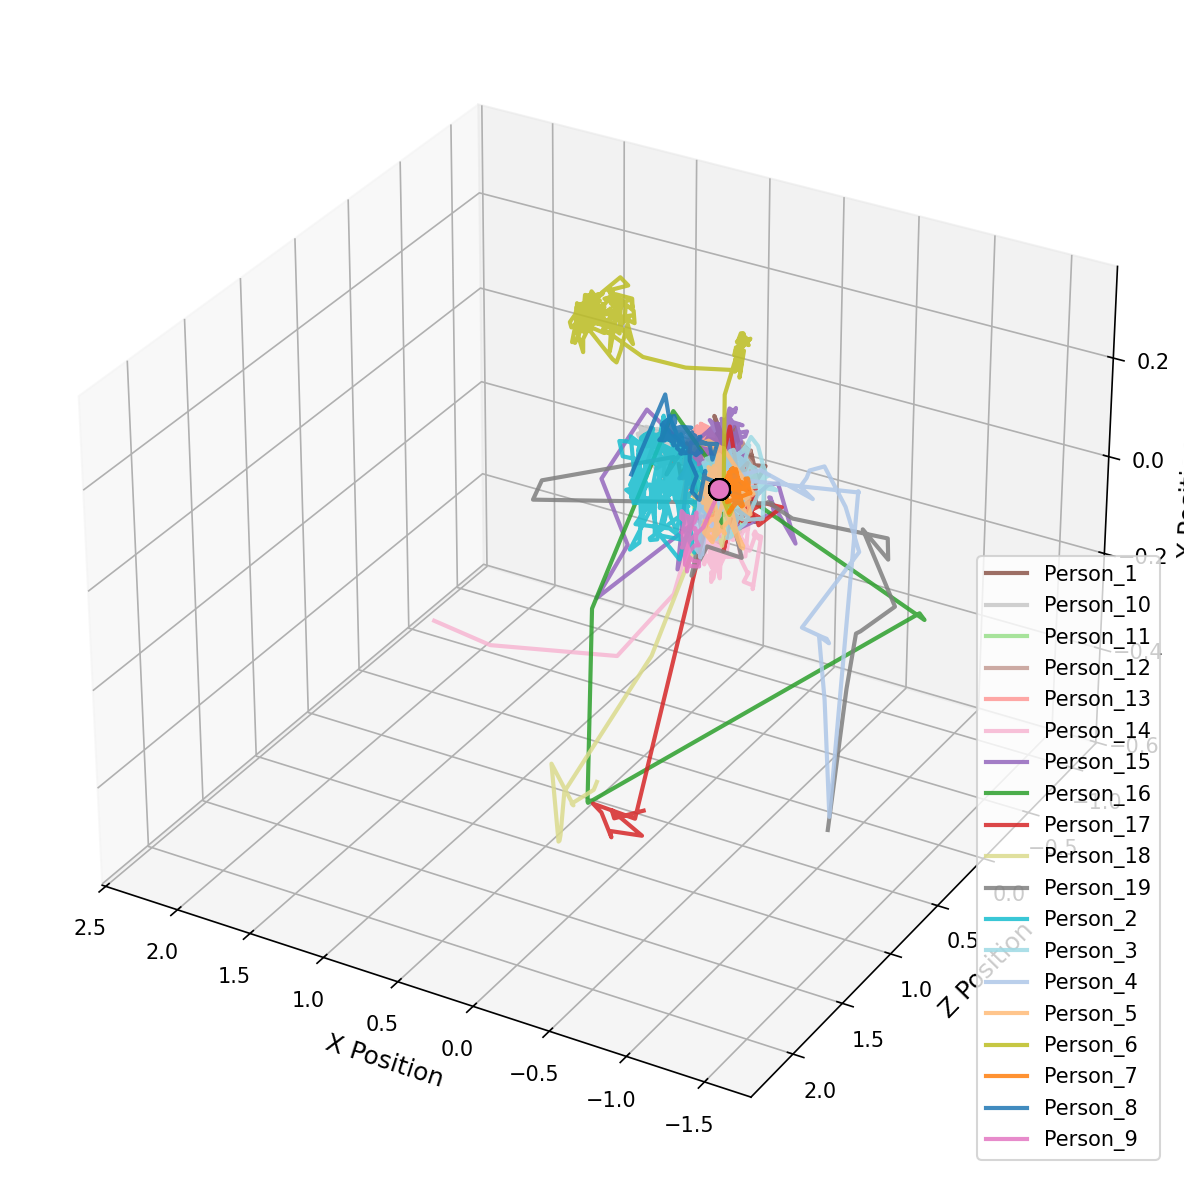
\includegraphics[width=\textwidth]{comparison_A_scenarios_3d.png}
        \caption{Scenariul A}
        \label{fig:Scenariul A}
    \end{minipage}
    \hfill
    \begin{minipage}{0.32\textwidth}
        \centering
        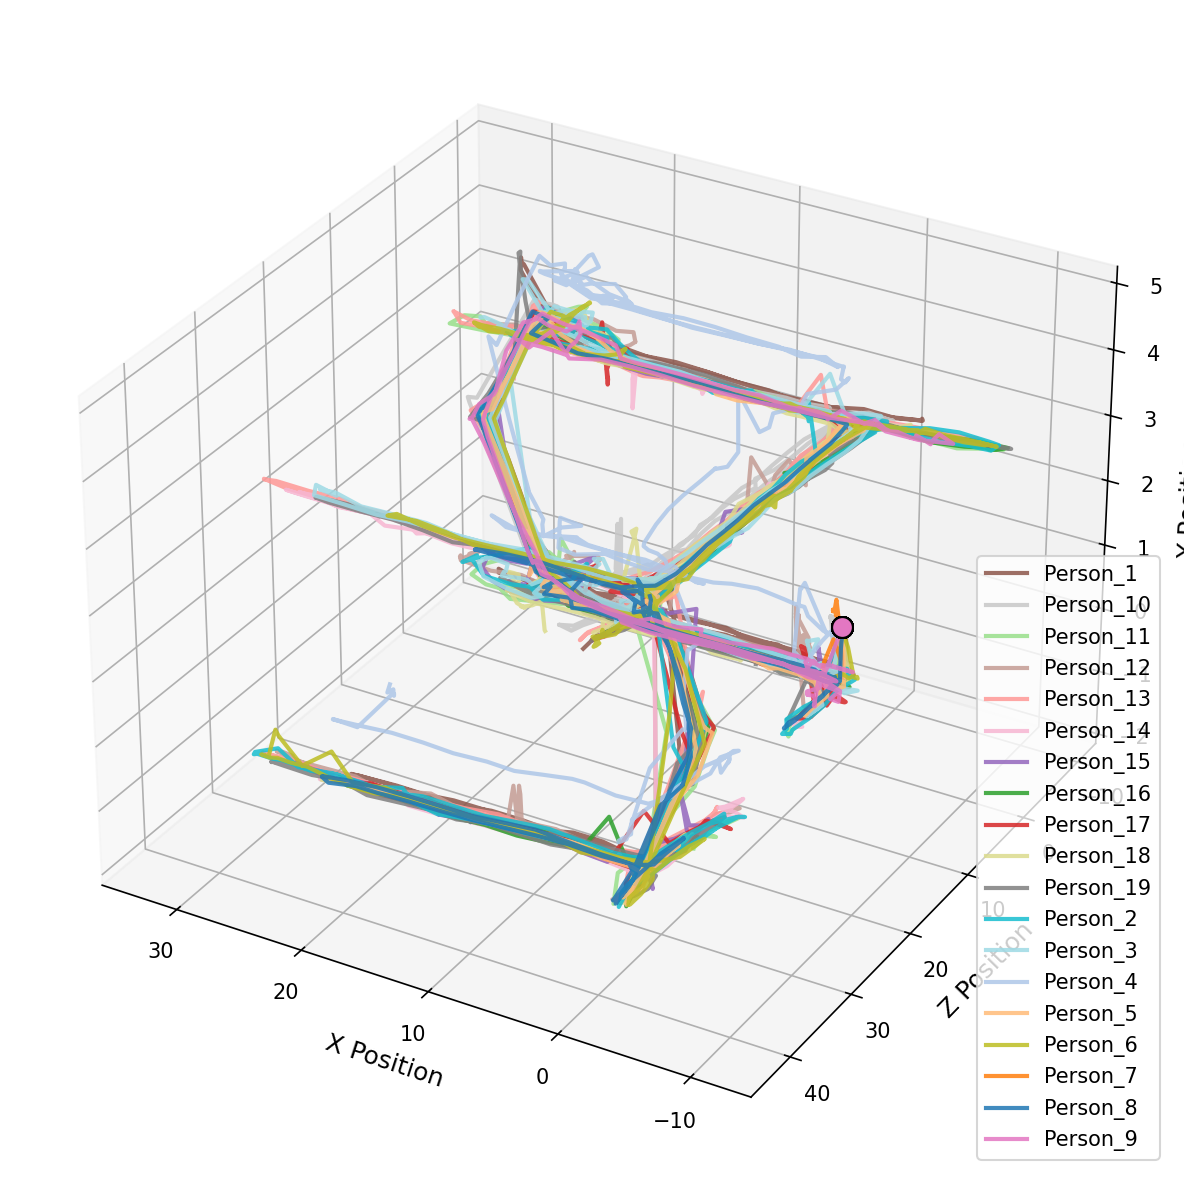
\includegraphics[width=\textwidth]{comparison_B_scenarios_3d.png}
        \caption{Scenariul B}
        \label{fig:Scenariul B}
    \end{minipage}
    \hfill
    \begin{minipage}{0.32\textwidth}
        \centering
        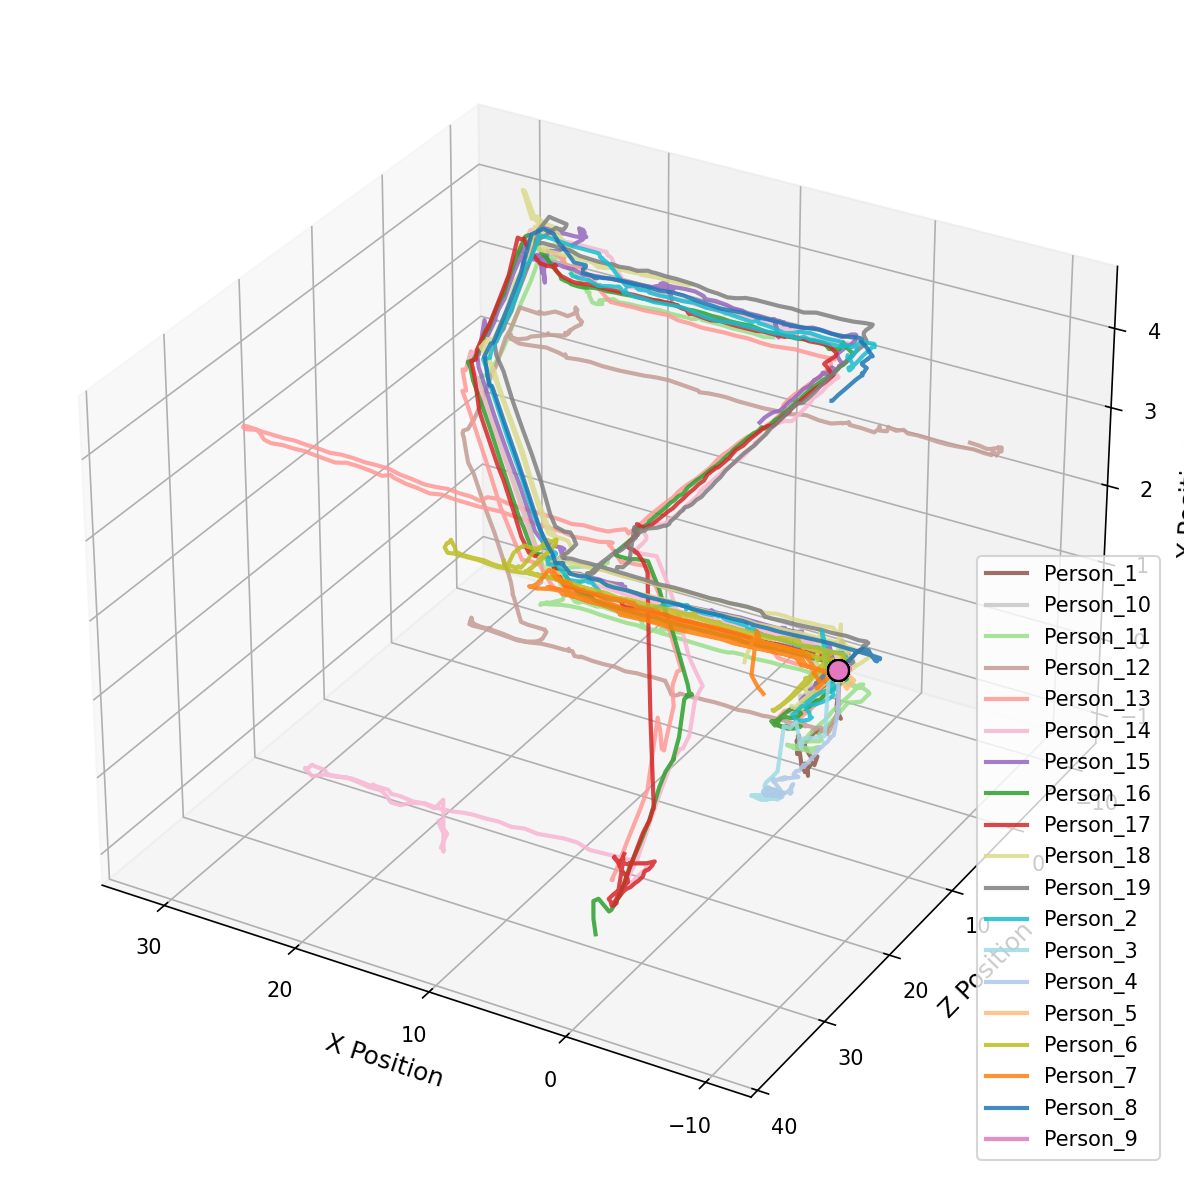
\includegraphics[width=\textwidth]{comparison_C_scenarios_3d.png}
        \caption{Scenariul C}
        \label{fig:Scenariul C}
    \end{minipage}

    \caption{(a) Scenariul A, (b) Scenariul B, (c) Scenariul C – vizualizare comparativă 3D a traiectoriilor de mișcare a capului pentru toți participanții.}
    \label{fig:Comparatie pe scenarii}
\end{figure}


\subsection{Indicele cantitativ de atipicitate și generare automată de raportare}

Așa cum este ilustrat în graficul \ref{fig:Clasament global}, analiza eșantionului relevă o distribuție structurată în trei categorii, cu grupul de variație ridicată (peste 0.70) care identifică cele mai semnificative divergențe comportamentale. Person\_7 și Person\_9 reprezintă principalele valori extreme (outliers), prezentând cele mai mari distanțe Mahalanobis și scoruri de consistență. Deși Person\_8 depășește de asemenea acest prag, analiza anterioară îl identifică drept o abatere determinată de energie de mișcare excepțională, mai degrabă decât de lipsă de control.

Intervalul de variație medie (0.50–0.70) cuprinde majoritatea grupului analizat, incluzând cazuri limită (Person\_4 și Person\_12), precum și mai multe profiluri tipice ale căror scoruri reflectă niveluri ridicate de implicare în mediul virtual. În schimb, grupul de variație redusă (0.30–0.50) conține cei mai centrați comportamental participanți, Person\_6 obținând cel mai mic scor, confirmând statutul său de centroid normativ al setului de date.

Distribuția evidențiază o structură clar bimodală, unde un decalaj numeric semnificativ separă outlierii principali de restul eșantionului. Această separare sugerează că indivizii cu scoruri maxime aparțin unei categorii comportamentale calitativ diferite față de grupul normativ. Dincolo de aceste extreme, algoritmul a identificat un cluster mare și omogen care reflectă un standard consistent de mișcare stabilă. Absența scorurilor sub 0.3 indică faptul că fiecare participant a menținut un nivel de bază de distinctivitate individuală în mediul VR. În final, contrastul dintre convergența grupului și profilurile atipice izolate validează sensibilitatea modelului în detectarea anomaliilor fundamentale de mișcare.

\begin{figure}[H]
    \centering
    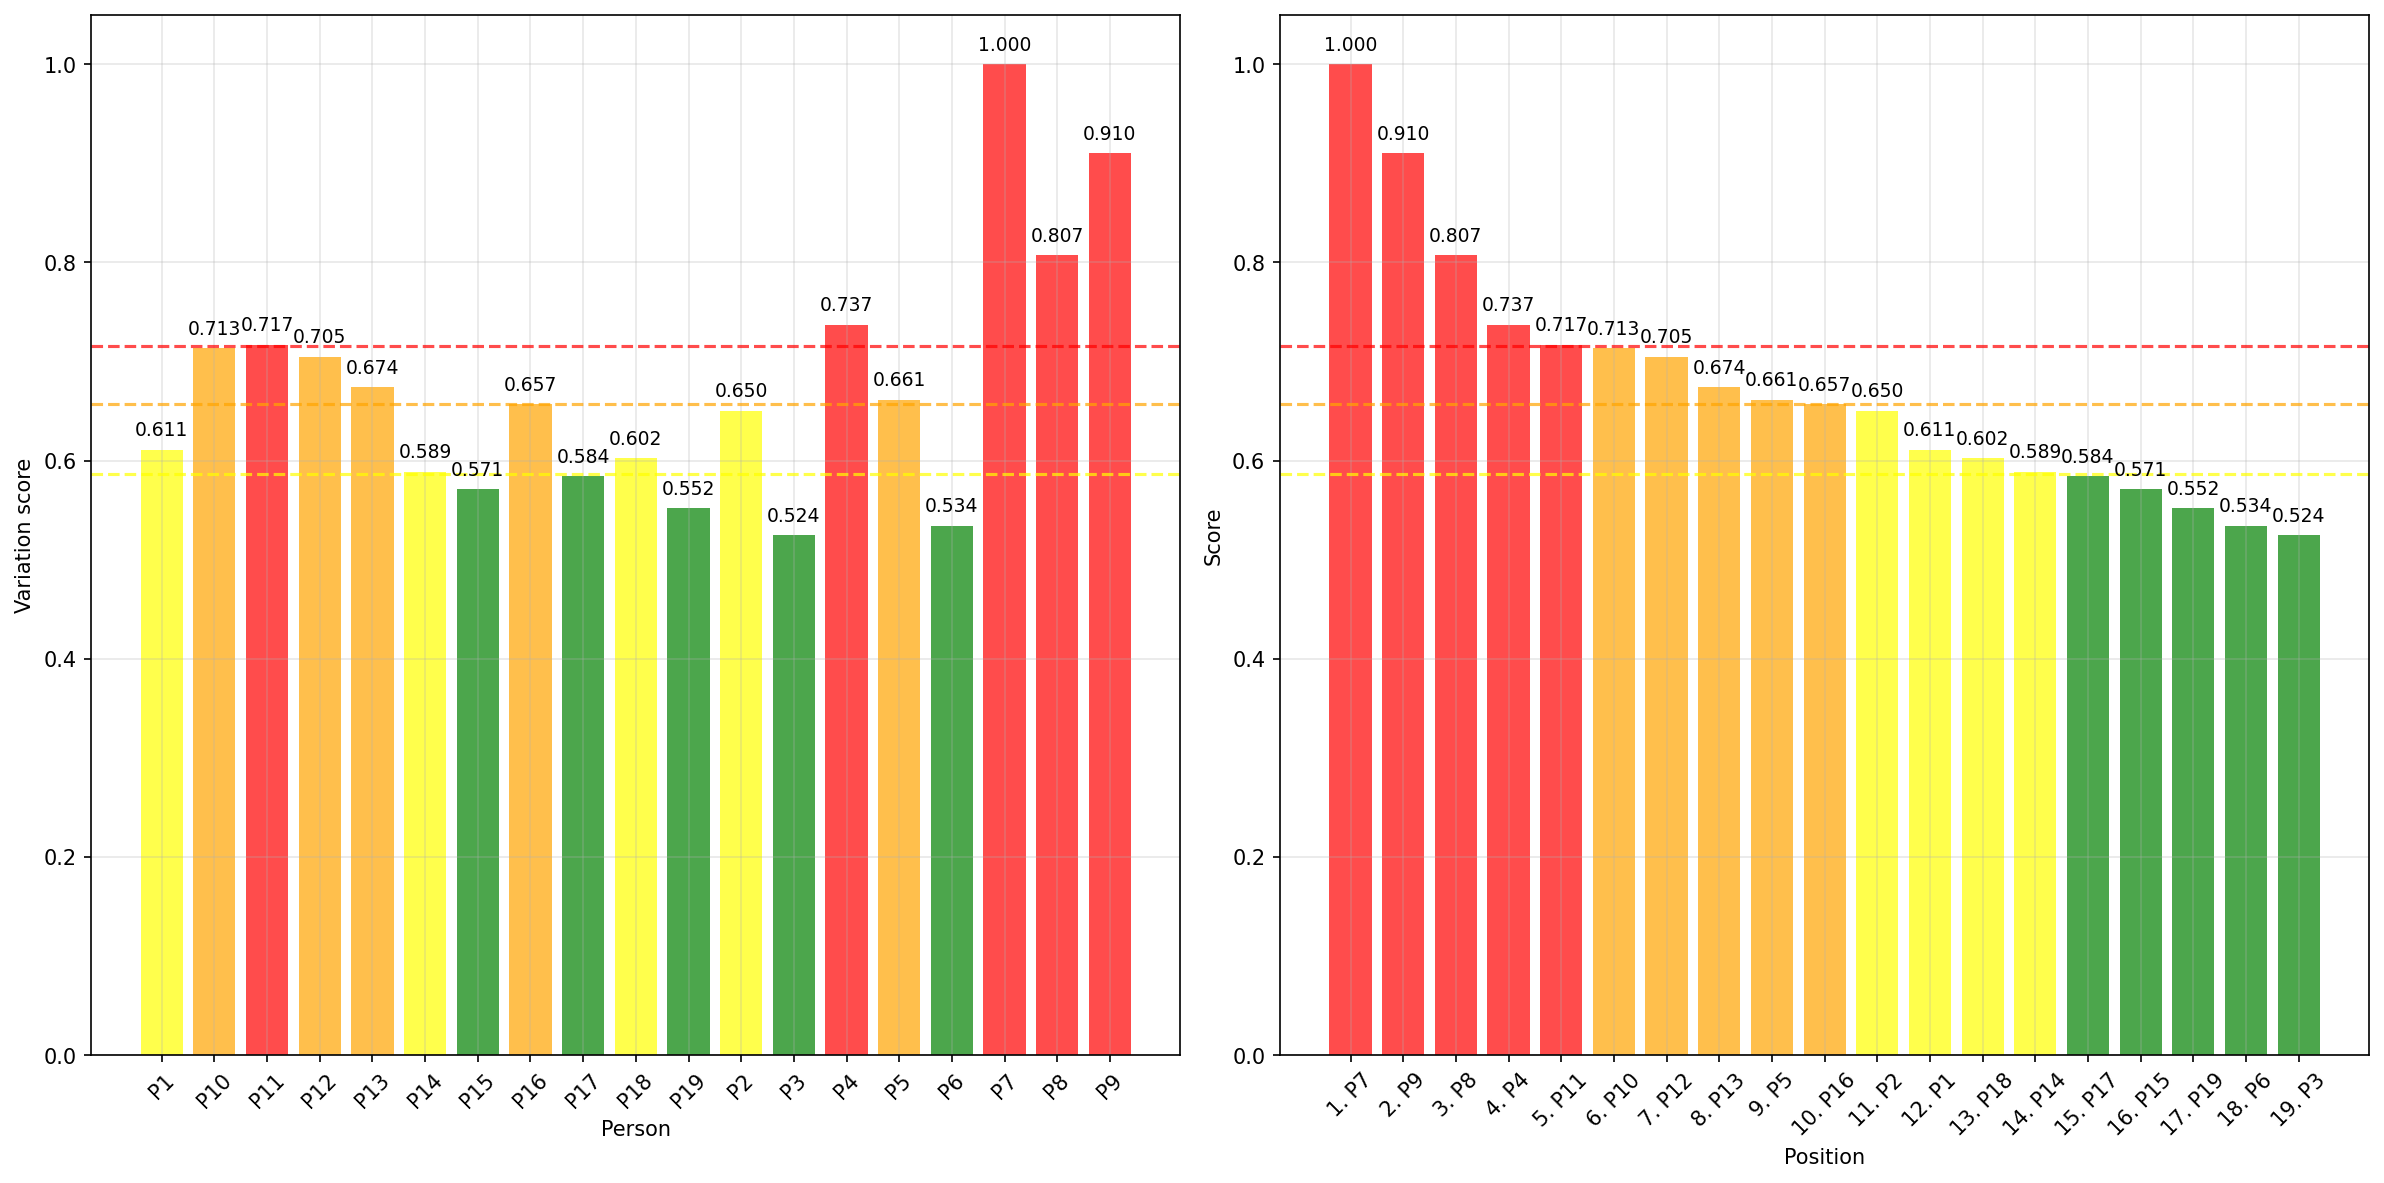
\includegraphics[width=0.5\linewidth]{behavioral_variation_report.png}
    \caption{Clasament global al atipicității.}
    \label{fig:Clasament global}
\end{figure}

% Comparatia cu abordari existente -> solutii diferite, implementari diferite, avantaje, dezavantaje

% structura generala a aplicatiei, functionalitati, diagrama cazuri de utilizare, detalii de implementare



% OBIECTIVA

\chapter{Concluzii și direcții viitoare}

Acest studiu a abordat provocarea identificării și clasificării tiparelor comportamentale în VR pentru a determina corelația acestora cu dizabilitățile motorii fizice.

Metodologia noastră a utilizat inițial clusterizare ierarhică aglomerativă pentru a genera dendrograme, oferind o vizualizare transparentă a modului în care grupările comportamentale naturale apar din date brute. Ulterior, am dezvoltat o metodă analitică mai complexă, bazată pe PCA pentru reducerea dimensionalității, pe clusterizare K-means și pe un scor compozit pentru cuantificarea atipicității.

Rezultatele demonstrează că metoda propusă a detectat cu succes toți participanții cu dizabilități motorii, mapând cu acuratețe limitările specifice ale acestora, cum ar fi restricția verticală observată la Person\_7 și orientarea persistent descendentă a capului la Person\_9.

Totuși, analiza a evidențiat și o provocare semnificativă: sistemul a etichetat ca atipici și unii participanți ale căror profiluri comportamentale, la inspecție calitativă, reflectă un nivel ridicat de implicare spațială, mai degrabă decât restricții motorii. În mod notabil, Person\_8 a obținut un scor ridicat de variație (0.72), determinat de o explorare extrem de energică a mecanismelor de tip gaze-block și de o activare extinsă a zonei superioare, atingând gama verticală maximă.

Acest lucru indică faptul că algoritmul are dificultăți în a distinge între atipicitatea generată de un nivel ridicat de implicare și curiozitate, și atipicitatea generată de restricțiile de navigație caracteristice deficiențelor motorii. Lucrările viitoare se vor concentra, prin urmare, pe dezvoltarea unui strat interpretativ secundar care să rafineze clasificarea, prin separarea deficiențelor funcționale de comportamentele extreme, dar sănătoase, de tip explorator.

% Sinteza rezultatelor -> ce a functionat, care au fost dificultatile, cum au fost depasite, lista de probleme deschise

% Directii viitoare -> probleme ramase deschise, idei de abordare

\addcontentsline{toc}{chapter}{Bibliografie}
\printbibliography

% !cel putin 5 titluri 

\appendix

\section*{Anexe}

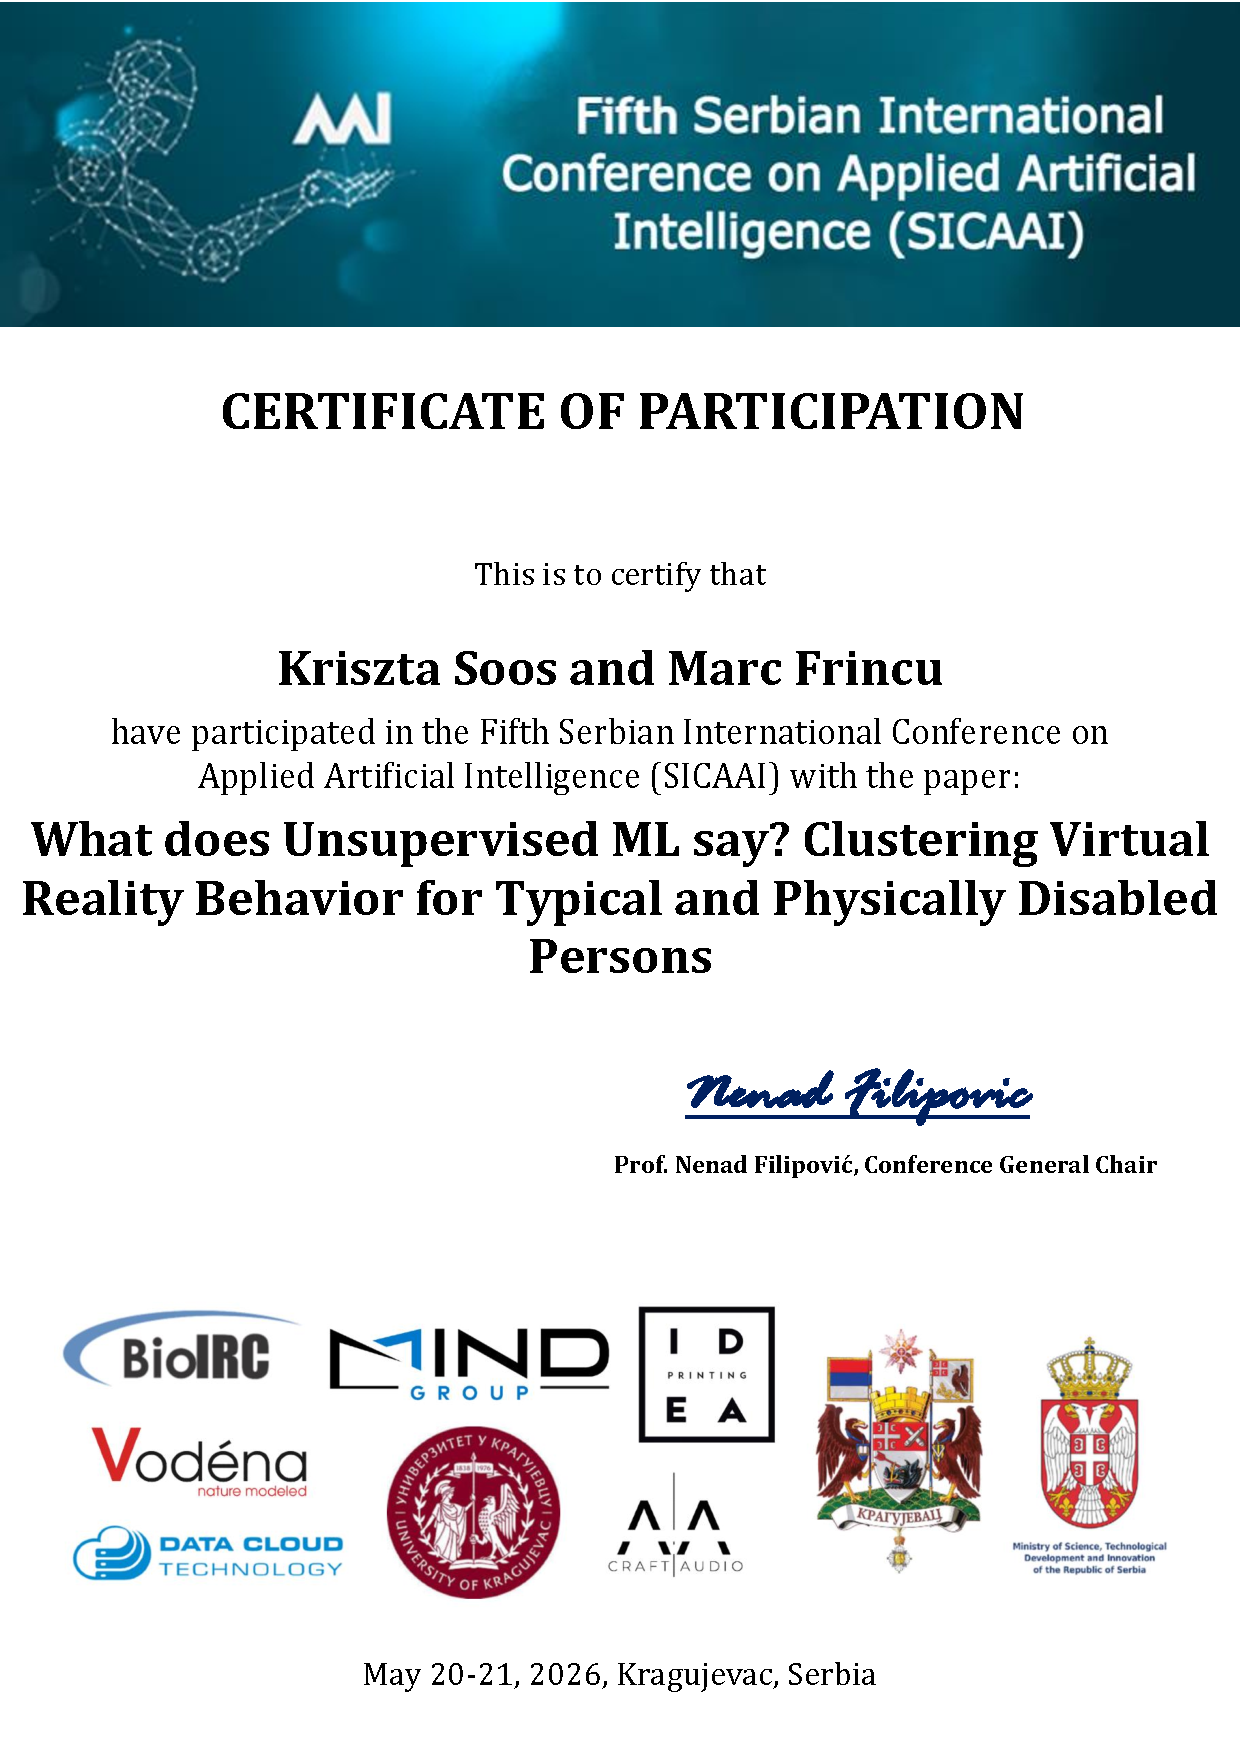
\includepdf[pages=-]{AAI2026 Kriszta Soos.pdf}

\end{document} 